\ifpdf
	\graphicspath{{5/pic/PNG/}{5/pic/PDF/}{5/pic/}}
\else
	\graphicspath{{5/pic/EPS/}{5/pic/}}
\fi

\chapter{Neutronics modules}\label{chap:hermes}

As we have seen in \cref{chap:nte-methods}, the various transport approximations lead to coupled systems of differential
equations with finite element approximations formulated on product spaces. In order to implement these models into a
practical solution method, it is thus necessary to appropriately deal with the coupling of variables. 

In standard finite element
assembling procedures, we would need to use the same underlying mesh $\mesh$ and approximation space $\Space_{hp}$ for
all components of the solution (which, given the large differences in the behavior of the studied fields like group
fluxes, directional fluxes, or angular flux moments, means a significant waste of computational resources) or use some
form of data interpolation to evaluate integrals of type 
\begin{equation}\label{eq:mixed_int}
	\int_{\elem\in\mesh} \sigma_s^{gg'} u^g v^{g'}\,\d{\br}
\end{equation}
(as appearing for instance in the multigroup diffusion approximation) when $u^g$ and $v^{g'}$ do not live on the same
mesh. To avoid this interpolation and errors associated with it, the C++ finite element library Hermes2D uses the
original \textit{multimesh assembling} approach \cite{Hermes-thermoelasticity}. 

To illustrate Hermes2D capabilities for efficiently solving coupled PDE systems, we will consider the general form of
both the multigroup diffusion and $\SPN$ problems as discussed in \sref{sec:sp3_weak}, i.e. the general form of Problem
\ref{prb:sp3} (or, equivalently, \ref{prb:sp3bis}). As we are interested here in its finite element approximation, we
start by writing the restriction of this general weak problem to the approximation subspace constructed in such a
way that each component of the solution can be approximated by different set of basis functions:
$$ 
	\mathbb{V}_{hp} \equiv \mathbb{V}_{hp}(\VV) = \prod_{j=1}^M \Space_{j}^{hp}(\VV) \subset \mathbb{H}(\VV),
$$
where the component-specific spaces $\Space^{hp}_{j}$ will be substantiated below. \\
\begin{problem}\label{prb:general}
Given $\mathrm{Q} = \colset{q_i}{M} \in \left[\Lp[2](\VV)\right]^M$, find $\U_{hp} = \col \{u_{j}^{hp}\}_M \in
\mathbb{V}_{hp}$ such that
\begin{equation}\label{eq:weak_general}
\begin{gathered}
	a(\U_{hp}, \mathrm{V}) = f(\mathrm{V}) \quad \forall \mathrm{V}\in \mathbb{V}_{hp},\\[.3em]
	a(\mathrm{U}, \mathrm{V}) := \int_{\VV} \bigl(\mat{D}\nabla\mathrm{U} : \nabla \mathrm{V} +
	\mat{C} \mathrm{U}\cdot\mathrm{V}\bigr)\d{\br} +  \int_{\pV} \gamma\mat{G}\mathrm{U}\cdot\mathrm{V}
	\,\d{S},\\
 	f(\mathrm{V}) := \int_{\VV}\mathrm{Q}\cdot\mathrm{V}\,\d{\br},\quad \bigl(\mat{D}\nabla\mathrm{U}\bigr) : \nabla
 	\mathrm{V} = \sum_{j=1}^M\sum_{\alpha=1}^3 D_j\pd{u_j}{x_\alpha}\pd{v_j}{x_\alpha}
\end{gathered}
\end{equation}
where the diagonal matrix $\mat{D}$ and matrices $\mat{C}$ and $\gamma\mat{G}$ are defined in \eqref{eq:SP3_mat} and
Appendix \ref{app:SPN} for the  $\SPN[3,5,7]$ models and in \eqref{eq:dif_mat} for the multigroup diffusion ($\SPN[1]$)
model. As discussed in \sref{sec:sp3_weak}, eq. \eqref{eq:weak_general} can be put into an equivalent form \\[.2em]
\begin{equation*}
\begin{matrix}
		\a{1}{1} 	& + & \b{1}{2} 	& + & \cdots 	& + & \b{1}{M} 	& = & \l[1], &\forall v_1\in \Space_{1}^{hp}, \\[.35em]
		\b{2}{1} 	& + & \a{2}{2} 	& + & \cdots 	& + & \b{2}{M} 	& = & \l[2], &\forall v_2\in \Space_{2}^{hp}, \\[.35em]
		\vdots 		& 	& \vdots 		& 	&	\ddots	& 	&	\vdots 	 	& = & \vdots\\[.35em]
		\b{M}{1} 	& +	& \b{M}{2} 	& +	& \cdots 	& +	&	\a{M}{M} 	& = & \l[M], &\forall v_M\in \Space_{M}^{hp}
\end{matrix}
\end{equation*}\\[.5em]
where for $i,j = 1,2,\ldots, M$,\\[.5em]
\begin{equation*}
 	a_{ij}(u,v) := \int_{\VV} \bigl({D}_{ij}\nabla u \nabla v +
	C_{ij} u v \bigr)\d{\br} + \int_{\pV} \gamma G_{ij} u v
	\,\d{S},\quad
 	f_{i}(v) := \int_{\VV}q_i v\,\d{\br}.
\end{equation*}
\end{problem} 

\newpage
\section{Multimesh hp-FEM}
\comment{
Consider the multigroup neutron diffusion problem in a typical thermal reactor with heterogeneous core.
As the neutron flux in lower energy groups (fast neutrons) is generally much smoother than flux in higher energy groups 
(slow neutrons), it makes sense to approximate each group on its own mesh and approximation space. Analogous situation 
arises in the mono-energetic $\SPN[5]$ problem -- as we will see in the examples below, the three $\SPN[5]$ moments 
$\phi^s_0$, $\phi^s_2$, $\phi^s_4$ generally behave very differently and the ability to approximate each moment 
independently can greatly save computational resources.} 



Let us define a set of meshes 
$$ \meshgen{j} = \{\elem_j\},\quad
	\overline{\VV} = \bigcup_{\elem_j\in\meshgen{j}} \overline\elem_j.
$$
We assume that the meshes originated from a common \textit{master mesh} $\meshgen[m]{}$ by successive refinements
(independent for each mesh), but are otherwise arbitrary. The corresponding approximation
spaces are given by
\begin{equation}\label{eq:hermes_space}
	\Space^{hp}_j = \left\{v^{hp}_j \in C^0(\VV): \left. v^{hp}_j\right\vert_{\elem_j} \circ\, \mathfrak{r}_j \in
	\mathcal{P}_{p}(\hat{\elem}),\ \elem_j\in\meshgen{j}
	\right\}
\end{equation}
where $\hat{\elem}$ is the reference element (unit square or right triangle in Hermes2D), $\mathfrak{r}_j :
\elem_j \to \hat{\elem} $ maps the physical element in $g$-th mesh to the reference element and
$\mathcal{P}_{p}(\hat{\elem})$ is the space of polynomials of degree up to $p$ (tensor product polynomials in case of
$\elem$ being a quadrilateral). We will refer to the highest degree $p$ of the polynomial contained in the approximation
space as to the approximation order of that space. In Hermes2D, the meshes can contain both
triangular and quadrilateral elements. In order to prevent conditioning of the standard finite element stiffness matrices from blowing up with
increasing polynomial degree, hierarchical shape functions are used to construct the approximation spaces \eqref{eq:hermes_space} in
preference to the usual Lagrangian nodal basis (\cite[Sec. 2.5.3]{Hermes-book2}). In the case of a quadrilateral
mesh, for instance, $\Space^{hp}_j$ is composed of functions that are on the unit square $\hat\elem$
\begin{enumerate}
	\item[(a)] $p \geq 1$: bilinear functions with value $1$ in exactly one vertex of $\hat\elem$ and $0$
	in the remaining vertices,
	\item[(b)] $p \geq 2$: 2D polynomials with nonzero values on exactly one edge of $\hat\elem$ and vanishing on the
	remaining edges,
	\item[(c)] $p \geq 4$: 2D polynomials with nonzero values in the interior of $\hat\elem$ and vanishing on
	$\partial \hat\elem$.
\end{enumerate}
(see \fref{fig:bazep}).

\begin{figure}[!htb]
  \centering
  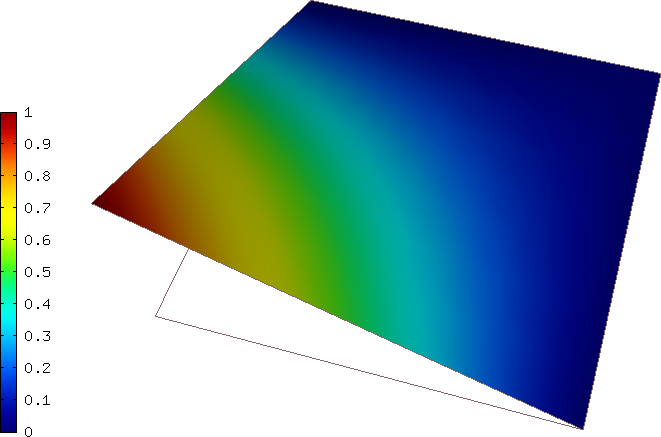
\includegraphics[width=.45\textwidth]{vtx}\hspace{.05\textwidth}
  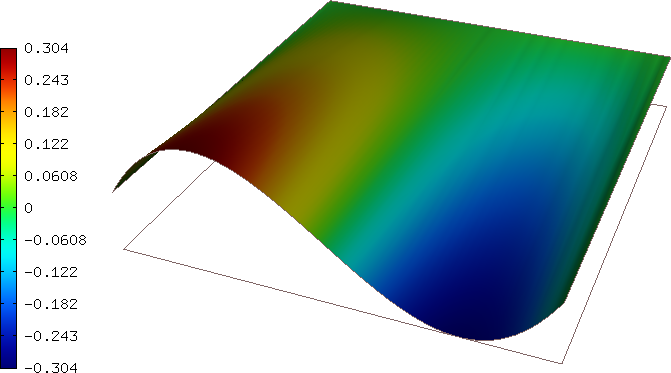
\includegraphics[width=.45\textwidth]{face}\\[1em]
  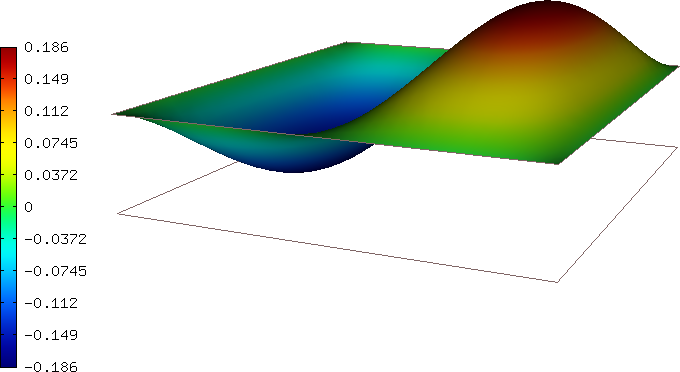
\includegraphics[width=.45\textwidth]{bubble}
  \caption{Shape functions of type (a), (b), (c).}
 	\label{fig:bazep}
\end{figure}

Note that the local approximation subspaces associated with each quadrilateral element might possess different
approximation orders in the lateral and longitudinal direction (as they are defined by a tensor product of 1D
polynomials in these two directions).
Moreover, approximation orders may also vary from element to element, i.e. for each $j$, $\Space^{hp}_j$ is decomposed into
\begin{equation*}
	\Space^{hp}_{j,\elem} = \{v^{hp}_j \circ\, \mathfrak{r}_j \in
	\mathcal{P}_{p_j}(\hat{\elem})
	\},\quad \elem_j\in\meshgen{j},\quad p_j = p(\elem_j)
\end{equation*}
the local approximation subspaces constructed so that the minimum rule for \mbox{$H^1$-conforming} approximations
(\cite[\S3.5.5]{Hermes-book1}) -- namely that the approximation order of these subspaces coincides with the
approximation order in element interiors (thus constraining the polynomial degree of the edge shape functions during
assembling) -- is satisfied. We will henceforth identify an element with the local approximation subspace
constructed on top of it, so that we can speak of element orders, etc.

Lastly, hanging nodes (mesh vertices in edge interiors) are also
allowed in $\meshgen{j}$ for greater flexibility of mesh adaptivity (and $H^1$ conformity recovered by additional constraints on the edge shape functions as
described in \cite[\S3.6]{Hermes-book1} and \cite{Hermes-hanging-nodes}).

\subsection{Multimesh assembling}
We are now ready to describe the basic principle of the multimesh assembling algorithm. This has been nicely done in 
the original paper \cite{Hermes-thermoelasticity} (which we will closely follow) but we include the brief description
here as well as it is directly related to one of author's own contributions to Hermes2D described in
\sref{sec:hermes_dg}.

In order to assemble mixed integrals of type \eqref{eq:mixed_int}, the assembling procedure works with a geometrical
union $\meshgen[u]{}$ of all meshes $\meshgen{1}$, $\meshgen{2}$, $\meshgen{3}$. This union is never explicitly created in
memory. Rather, its virtual elements are traversed by the usual element-wise assembling loop. Let $\widetilde\elem \in
\meshgen[u]{}$ be the currently visited virtual element. 
\begin{figure}[!hb]
  \centering 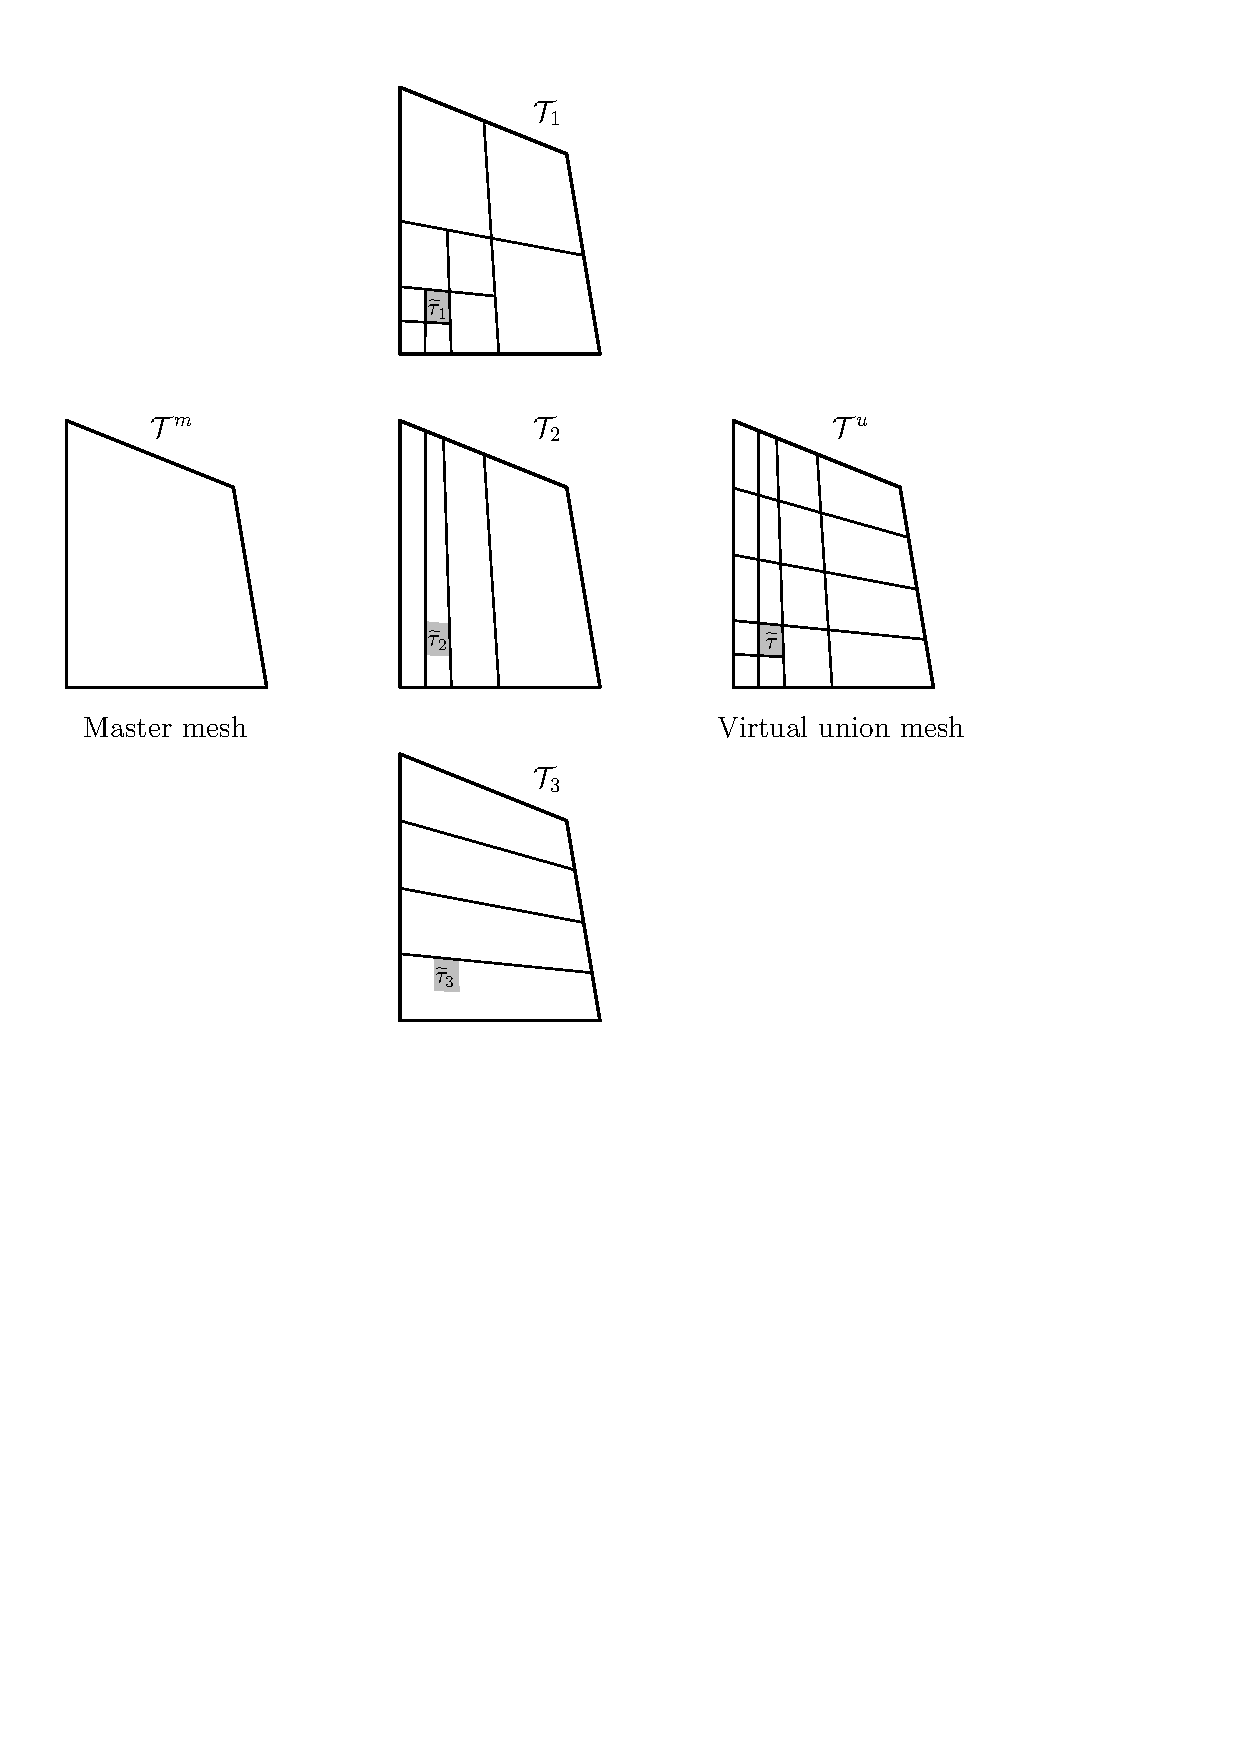
\includegraphics[scale=.775]{multimesh} \caption[Multimesh assembling]{One state of the multimesh
  assembling algorithm. Note that the sub-element mapping $\mathfrak{s}_1$ is identity.}
 	\label{fig:multimesh}
\end{figure}
As all meshes $\meshgen{j}$ originate from a common master
mesh, there is for each $j$ exactly one element $\elem_j\in\meshgen{j}$ such that $\widetilde\elem_j\subset \elem_j$ is
the \textit{sub-element} of $\elem_j$ (which is called in this context the \textit{active element} on $\meshgen{j}$)
corresponding to $\widetilde\elem$.


To evaluate the integrals comprising the weak formulation, each
sub-element needs to be transformed to the reference element where the appropriate quadrature points are defined.
While for the active element on $\meshgen{j}$, the referece mapping $\mathfrak{r}_j(\elem_j) = \hat{\elem}$ as required, it
transforms the sub-element to a subset $\mathfrak{r}_j(\widetilde\elem_j) \subset \hat{\elem}$. Thus another mapping
$\mathfrak{s}_j : \hat{\elem} \to \hat{\elem}$ is introduced (the \textit{sub-element mapping}) such that
$\mathfrak{s}_j(\mathfrak{r}_j(\widetilde\elem_j)) = \hat{\elem}$. These two mappings allow Hermes2D to evaluate all
integrals in the weak forms by using elements only on the mesh on which the integrands live, thus incurring no further
error beyond the inevitable one of numerical integration.

\subsection{Discontinuous Galerkin assembling}\label{sec:hermes_dg}
As a joint effort of the author of this thesis and Luk{\' a}{\v s} Korous, at this moment (November 2014) the main
developer of the Hermes2D project, Hermes2D has been enabled for discontinuous Galerkin approximation of
variational problems. This involved the extension of the assembly procedure to
perform surface integration over all edges of all elements for user-defined discontinuous Galerkin bilinear and linear
forms and also exposing for these forms the access to shape functions and geometrical information of both elements sharing a
common interface (thus allowing the user to define interface operators like $\jump{\cdot}$ and $\langle\cdot\rangle$ introduced in
 \sref{sec:DGM}). 
 Because of the possibility of hanging nodes in the mesh (essentially needed for efficient mesh
 refinement), the actual integration of these forms along element edges is non-trivial as matching points
 from both sides of the edge need to be correctly determined.  
This functionality has been implemented in the class \lstinline{NeighborSearch} based on the same fundamental idea
underlying the multimesh assembling (namely that of sub-element mappings).

The \lstinline[basicstyle=\ttfamily]{NeighborSearch} class characterizes a neighborhood of a given edge in terms of adjacent
elements and provides methods for getting limit values of discontinuous functions from both sides of the edge. Each instance of the
class is connected to a mesh and its active element. The current active element becomes the \textit{central element} of
the neighborhood and all adjacent elements the \textit{neighbors}. In order to search for the neighboring elements, one
selects a particular edge of the central element and calls a function that enumerates the neighbors and fills in the
array of sub-element mappings (transformations) necessary for getting function values at matching quadrature points
from both sides of the selected (active) edge.
The actual procedure depends on the relative size of the central element with respect to the neighbor element(s) across
the active edge:
\begin{itemize}
  \item If active edge is shared by two elements of same size, then the neighboring element is identified directly and 
  no additional transformations are needed to obtain values of any given function from either side of active edge.
\begin{figure}[!ht]
  \centering
  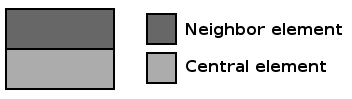
\includegraphics[scale=.45]{no_trans}
  \caption{Neighbor search -- ``no transformation'' case}
\end{figure}
  
  \item If the neighbor element is bigger than the central element, then we "go up" on the central element, until we
  find its parent that has the same size as the neighbor. We keep track of the visited intermediate parents and after 
  the final one has been found (in the ultimate case an element of the master
  mesh), we use them in reverse order to fill in the sub-element mapping array. These
  transformations will be applied to integration points used when integrating a function on the neighboring
  (bigger) element in order to obtain values at points matching those from the central element's side.
  
\begin{minipage}{\linewidth}
    \centering
    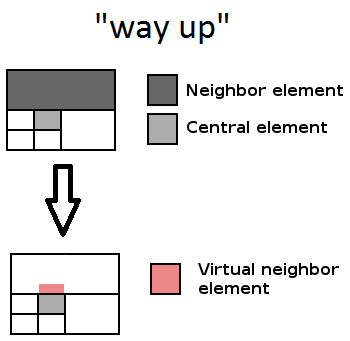
\includegraphics[scale=.6]{way_up2}
    \captionof{figure}{Neighbor search -- ``way up'' case}
\end{minipage}
  
  \item If the neighbor element is smaller than the central element, it means that it is one of several neighbors across
  the active edge. Hence, we "go down" in the central element in order to find a (virtual) sub-element matching the 
  currently processed neighbor and store the corresponding transformations in the neighbor's row of the
  (two-dimensional) array of sub-element mappings. This way, we obtain for each neighbor a set of
  transformations which will be applied on the central element to transform integration points to the correct
  sub-element matching the neighbor.

\begin{minipage}{\linewidth}
    \centering
    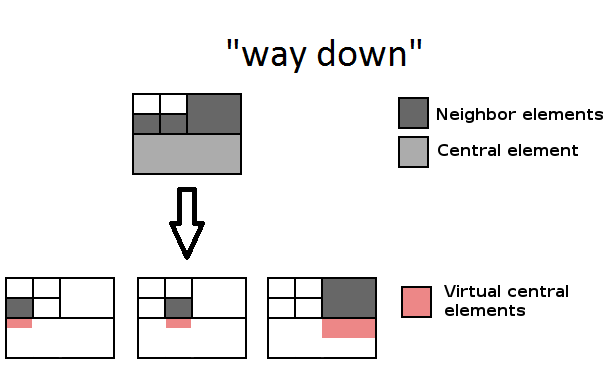
\includegraphics[scale=.6]{way_down2}
    \captionof{figure}{Neighbor search -- ``way down'' case}
\end{minipage}

\end{itemize}

If only an external function is supposed to be discontinuous across the active edge (e.g. in the case of assembling
linear forms), an appropriate \linebreak\lstinline[basicstyle=\ttfamily]{DiscontinuousFunc} object is created for such a
function and exposed to the user who can use it to retrieve actual values at the matching integration points from both
sides of the active segment.

If also the trial and test functions need to be considered discontinuous (e.g when assembling DG bilinear forms), the
local approximation bases (called \textit{shapesets} in Hermes2D) on the central element and on the current
neighbor element are extended by zero to the whole neighborhood of the two elements.
The so-called \textit{extended shapeset} thus created is 
queried during assembling for the count of all contained extended shape functions and their global DOF (degree of
freedom) numbers.
Assembling is done over all these extended shape functions -- the currently processed trial and test functions
is exposed to the user again as
\lstinline[basicstyle=\ttfamily]{DiscontinuousFunc} objects with the shape functions' values (and derivatives) at
integration points at both sides of active edge.
  
This procedure is limited by the requirement that the number of integration points at both sides of
active edge is the same. This is enforced artificially during assembling by performing the integrations of DG interface
forms using a quadrature of the maximal supported order. Note that this does not restricts the approximation spaces
in any way -- it only pertains to the numerical integration.

\section{$hp$-adaptivity}\label{sec:hermes_adapt}
The goal of the $hp$-adaptivity process is to combine spatial subdivision of selected elements ($h$-refinement) with
local increase of their approximation order ($p$-refinement) so that the total available number of degrees of freedom at
given stage of the process is utilized most efficiently (i.e., relatively big number of low-order elements is used in
regions with highly oscillating solution while smaller number of high-order elements in regions with smoother solution
behavior). As there are many possible combinations of $h$ and $p$ refinements of given element, one number per element
provided by traditional a-posteriori error estimates for FEM is insufficient to guide the $hp$ adaptivity. To circumvent
this issue, local error estimation in Hermes2D is based on comparing two solutions of different approximation orders --
a robust technique borrowed from the field of numerical solution of ordinary differential equations. In particular, it
allows to determine the whole shape of the approximation error $e = u - u_{hp}$ over each element and use it to determine the best
refinement candidate that decreases the total approximation error for the lowest number of added DOF.

For illustration, let us consider the general approximate problem \ref{prb:general}, coming from the corresponding exact
variational problem with solution $\U\in\mathbb{H}^1(\VV)$. Note that the approximation error is a vector-valued
function 
$$ 
	\Ehp = \U_{hp} - \U; 
$$ 
the total error can be measured by 
\begin{equation}\label{eq:measure}
\norm{\Ehp}^2 = a(\Ehp,\Ehp) =
	\sum_{i=1}^M\sum_{j=1}^M a_{ij}(\ehp{j}, \ehp{i}) = \sum_{i=1}^M \norm{\ehp{i}}^2, 
\end{equation}
which in the case of symmetric coercive bilinear form $a$ (single-group diffusion/$\SPN$ models) is the true energy norm
associated with the problem. In the non-symmetric case, \eqref{eq:measure} can still be used to measure the
approximation error and guide the adaptivity. This approach takes into account the coupling of the fields
(group-to-group coupling induced by scattering and/or the coupling between the $\SPN$ moments). Alternatively, one may
use the simpler $\mathbb{H}^1(\VV)$ norm  -- then
$$
	a(\U,\mathrm{V}) = (\U,\mathrm{V})_{\mathbb{H}^1(\VV)},\quad a_{ij}(u,v) =
	(u,v)_{H^1(\VV)}\kron{i}{j}
$$
and the $\mathbb{H}^1(\VV)$ norm of the total error is given by
$$
	\norm[1]{\Ehp}^2 = \sum_{i=1}^M \norm[1]{\ehp{i}}^2 = \sum_{i=1}^M (\ehp{i},\ehp{i})_{H^1(\VV)}.
$$

To guide the adaptivity process, the error is estimated by replacing the unknown exact solution $\U$ by a
\textit{reference solution} $\flfl_{\rf}$ approximating $\U$ using a greater number of degrees of freedom than
$\U_{hp}$. The adaptation algorithm consists of the following steps:

\begin{enumerate}
\item 
Given a set of spaces $\{\Space^{hp}_j\}_{M}$, a globally refined set $\{\Space^{h/2,p+1}_j\}_M$ is first
created and Problem \ref{prb:general} solved on these spaces, yielding $\flfl_{h/2,p+1} =: \flfl_{\rf}$. 

\item
The coarse
component of the approximation pair $(\U_{hp}, \flfl_{\rf})$ is then obtained as
$$
	\U_{hp} = \Projop[hp]\flfl_{h/2,p+1}.
$$
We still denote the error function defined via this approximation pair as $\Ehp$:
$$
	\Ehp = \U_{hp} - \flfl_{\rf} = \Projop[hp]\flfl_{h/2,p+1} - \flfl_{h/2,p+1}.
$$

\item
The local contribution of each element $\elem_i\in\meshgen{i}$ to the $i$-th component of the total error
$$ 
	\norm{\ehp{i}}^2 = \sum_{j=1}^M a_{ij}(\ehp{j}, \ehp{i}),\quad i = 1,2,\ldots, M 
$$ 
can now be computed during the multimesh assembly of the involved bilinear forms. Let us denote this contribution by
$\eta^{hp}_{\elem,i}$.

\item
Elements contributing the
most to the global error are marked for refinement (using a user-specified threshold). Note that elements of
\textit{all} meshes are considered, so that every element of every mesh in $\{\meshgen{i}\}_M$ is compared with all 
others.

\item For each element marked for refinement, a multitude of refinements is
tested, so that $\elem_i\in\meshgen{i}$ in space $\Space^{hp}_i$ gives rise to several candidate spaces
$\Space^{h'p'}_i$ (83 possibilities are tested for triangular elements as illustrated below and even
more possibilities arise in the case of quadrilateral elements by considering anisotropic refinements in longitudinal
and lateral directions -- for more details, we refer to \cite{Hermes-adaptivity,Hermes-hanging-nodes}).

\begin{minipage}{\linewidth}
    \centering
    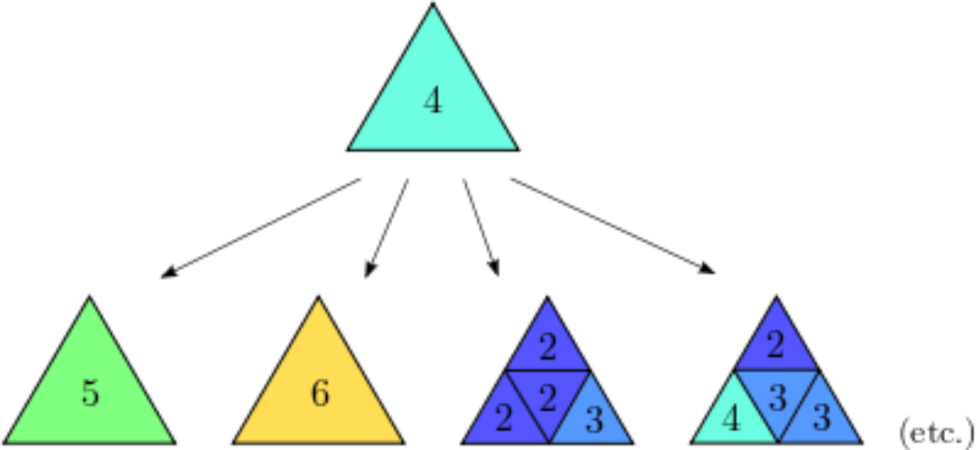
\includegraphics[width=4.5in]{refinements}
    \captionof{figure}[Refinement candidates of a triangular element]
    {Refinement candidates of a triangular element (number signifies the approximation order). From
  	\url{http://hpfem.org/wp-content/uploads/doc-web/doc-tutorial/src/hermes2d/D-adaptivity/intro-1.html}}
\end{minipage}

Error contribution $\eta^{h'p'}_{\elem,i}$ of each candidate is computed from the difference
$$
	 \Projop[h'p']\flfl_{h/2,p+1} - \flfl_{h/2,p+1}.	
$$

\item 
The refinement candidate that leads to the largest decrease of error for the associated increase of the number of DOF 
$$
	\frac{\log\left(\eta^{hp}_{\elem,i}\right) - \log\left(\eta^{h'p'}_{\elem,i}\right)}{\left(N_{\text{DOF}}^{h'p'} -
	N_{\text{DOF}}^{hp}\right)^\alpha}.
$$
where $\alpha$ is the customizable convergence exponent (set to $1$ by default), is finally selected and $\elem_i$ is
refined accordingly, ultimately leading to a set of adapted spaces for another iteration. The whole process is
terminated when the total error norm estimate $\norm{\Ehp}$ decreases below a user specified threshold.
\end{enumerate}

These steps represent a straightforward generalization of the so called \linebreak\mbox{projection-based}
$hp$-adaptivity \cite{Hermes-book2,demkowicz} to the multimesh setting. This approach is sufficiently general so that it can be
employed in solution of any type of PDE or their system. Also, pure $h$- or $p$-adaptivity can be realized by the same
algorithm. For an $h$-adaptive solution of simple elliptic equations, however, there exists a big
number of simpler and potentially more efficient approaches based on standard a-posteriori error estimates
\cite{gratsch}. One based on the estimate of the energy norm of the
error by the sum of the element residual and the jump of solution at element boundaries (computed using the actual 
approximation $\U_{hp}$) \cite{Kelly} has been also implemented into Hermes2D using the newly added discontinuous
Galerkin capability (needed for evaluating the jump terms) and will be used in example \sref{sec:stankovski}.

\subsection{Error estimator for $\SPN$ based on the scalar flux}\label{sec:errest}
As we are typically most interested in the scalar flux, we may use \eqref{eq:SPN_scalar_flux} to estimate the
error in scalar flux approximation for the $\SPN$ model (where we recall that $N$ is taken as odd integer):
\begin{equation}\label{eq:err-est-phi}
\begin{aligned}
	\norm[1]{\Ehp^{\phi}}^2 &= \left\Vert\suma[n]{0}{(N-1)/2}{F_{n}}\bigl(\phi^s_{2n} -
	\phi^{s,\text{ref}}_{2n}\bigr)\right\Vert_1^2 
	\leq  \left(\suma[n]{0}{(N-1)/2}\left\Vert F_{n}\bigl(\phi^s_{2n} -
	\phi^{s,\text{ref}}_{2n}\bigr)\right\Vert_1\right)^2\\
	&= \left(\suma[n]{0}{(N-1)/2} \norm[1]{F_{n} e^s_{2n}}\right)^2
	= \suma[m]{0}{(N-1)/2}\suma[n]{0}{(N-1)/2} F_{n}F_{m}\norm[1]{e^s_{2n}}\norm[1]{e^s_{2m}}\\
	&= \suma[m]{0}{(N-1)/2}\suma[n]{0}{(N-1)/2} a^\phi_{mn}(e^s_{2n}, e^s_{2m})
\end{aligned} 
\end{equation}
where $e^s_{2n} = \bigl(\phi^s_{2n} - \phi^{s,\text{ref}}_{2n}\bigr)$ and $a^\phi_{mn}(u,v) =
F_{n}F_{m}\norm[1]{u}\norm[1]{v}$.
This estimate will be used in the $\SPN$ examples in \sref{sec:ex_spn} to evaluate local element error contributions as
described in step 3 of the algorithm above.

\section{Neutronics modules and examples}
The author of this thesis has developed a multigroup $\SPN$/diffusion framework on top of Hermes2D that implements all
the basic building blocks of the weak formulation of Problem \ref{prb:general} for both transport approximations. It also allows
relatively simple specification of typical transport benchmarks, with automatic conversion between various possible sets
of specified cross-sections (basically implementing relations like \eqref{eq:st} in the multigroup approximation) and
calculating and visualizing basic quantities of interest like $\phi$, $\bJ$ and reaction rates. The $\SPN$ equation have
been implemented and tested up to $N = 9$, using the Mathematica script mentioned in App. \ref{app:SPN} that allows
simple extension to higher orders.

For solving the criticality eigenvalue problems of type \eqref{eq:discrete_eigenproblem}, the (inexact) inverse
iteration has been implemented according to paper \cite{Freitag}. It supports  both fixed and Rayleigh quotient shifting
and exact and inexact solves (with fixed or decreasing tolerance during the course of the eigenvalue iteration) of the
associated linear system in the $i$-th iteration:
$$
	(\mat{A} - s^{(i)}\mat{B})\mat{x}^{(i+1)} = \mat{B}\mat{x}^{(i)}, 
$$
where $s^{(i)}$ is the actual shift value. Combination of both shift types is possible as it may be generally
advantageous to perform several iterations with fixed shift (possibly zero, when the iteration reduces to the simple 
power iteration) and then to switch to variable shifting to speed-up the convergence rate.

In addition, the $\SN$ method has been also implemented to test the accuracy of the more approximate $\SPN$ and
diffusion models. This module uses and extends the neutronics classes developed for the $\SPN$ module (material
data specification, visualization, the class that encapsulates fixed-point iteration for both the
eigenvalue calculation and simple source iteration \eqref{eq:SI}, etc.) and implements the discontinuous Galerkin
spatial discretization as described in \sref{sec:snpnspatial}, using the multimesh DG assembler outlined in
\sref{sec:hermes_dg}. The ordinates set described in \sref{sec:ordinates} is implemented in the module (note that for
solving 2D problems to which Hermes2D is restricted, only $M/2 = N(N + 2) / 2$ ordinates in the upper hemisphere
$\Omega_z > 0$ need to be considered in constructing the $\SN$ system). As such, this ordinates set allows to accurately
represent reflective conditions at boundaries aligned with axes of the Cartesian coordinate system.

For the multigroup diffusion, this framework is available in the master branch of the current Hermes2D release.
The $\SPN$ version with various examples presented below is available from the local repository of the author and is 
based on an older version of Hermes:\\
\url{https://github.com/mhanus/hermes/tree/neutronics-master}.\\
The development version
mainly for testing the $\SN$ module (including additional $\SN$ examples) is available from\\
\url{https://github.com/mhanus/hermes/tree/SN-adaptive}.\comment{\\
Please note that unlike the neutronics framework
itself, the examples are not as regularly updated and thus some of them might not work in some of the branches
due to the rather precipitous evolution of the library that has involved many fundamental interface changes. 
}

\subsection{$\SPN$ and diffusion examples} \label{sec:ex_spn}

The following examples show the behavior of the $\SPN$ approximation and some features of Hermes2D and its
new neutronics modules. The use of adaptivity kept the sizes of these problems reasonably small so that a sparse direct
solver UMFPACK \cite{UMFPACK} could be used for their efficient solution. The calculations were performed on the Toshiba
Portege M750 laptop with Intel Core 2 Duo P8400 / \SI{2.26}{GHz} processor (\SI{3}{MB} L2 cache) and \SI{4}{GB}  DDR2
SDRAM. The operating system was Ubuntu 10.10 64bit.

\subsubsection{Benchmark IAEA EIR-1}\label{sec:iaea}
This classical neutronics benchmark of the International Atomic Energy Agency models an arrangement of four homogeneous
absorbing and scattering regions with dimensions \SI{30\times 25}{cm} placed at the center of a rectangular pool of
total width \SI{96}{cm} and height \SI{86}{cm} with vacuum outer boundary conditions. Isotropic external neutron source
is uniformly distributed in two of the regions as seen from \fref{fig:40} and the table \ref{tab:iaea-coef} listing the material properties of the regions.
\begin{figure}[!htb]
\centering
  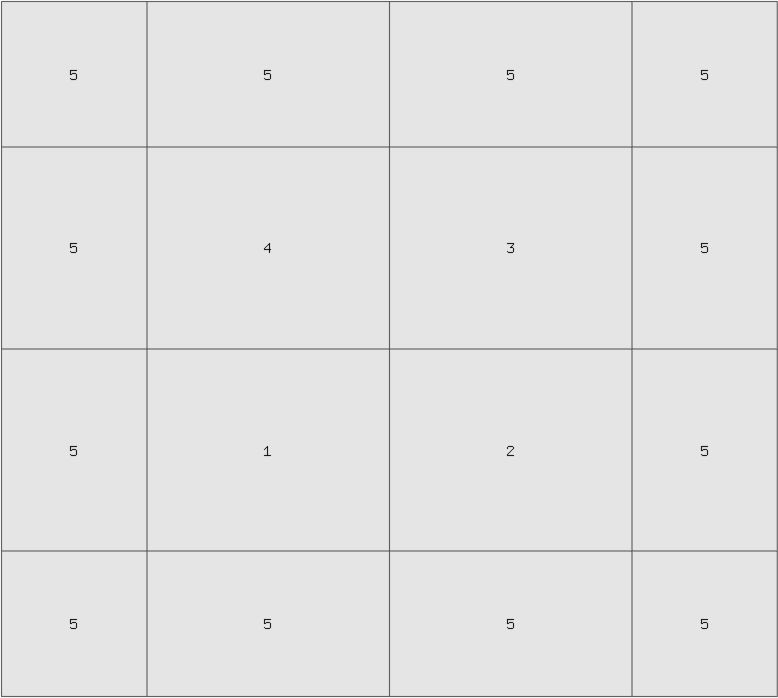
\includegraphics[scale=.2]{saphir/mesh.png}
  \caption[Initial mesh for the IAEA EIR-1 benchmark]{Initial mesh for the IAEA EIR-1 benchmark.}
  \label{fig:40}
\end{figure}

\begin{table}
\centering
	\begin{tabular}{c|ccc}
	  %\hline
		Region \# & $\sigma_t\ [\SI{}{cm^{-1}}]$ & $\sigma_s\ [\SI{}{cm^{-1}}]$ & q\ [\SI{}{cm^{-3}.s}] \\\hline
		1   & 0.60 & 0.53 & 1.0 \\[.2em] 
		2   & 0.48 & 0.20 & 0.0  \\[.2em] 
		3   & 0.70 & 0.66 & 1.0  \\[.2em] 
		4   & 0.65 & 0.50 & 0.0  \\[.2em] 
		5   & 0.90 & 0.89 & 0.0%  \\\hline  
	\end{tabular} 
\caption{Table of material properties for benchmark \ref{sec:iaea}}
\label{tab:iaea-coef}
\end{table}

\begin{figure}[!ht]
\centering
\subfigure[$\phi$]{
  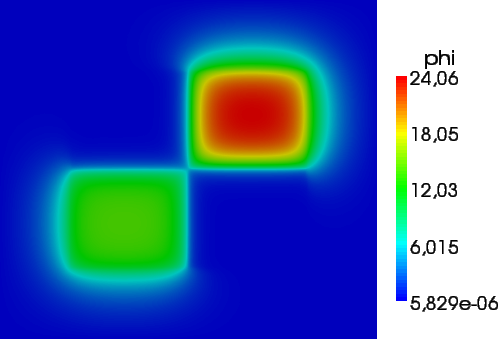
\includegraphics[width=.44\textwidth]{saphir/flux0p.png}
}
\hspace{1em}
\subfigure[$\phi_1^s$]{
  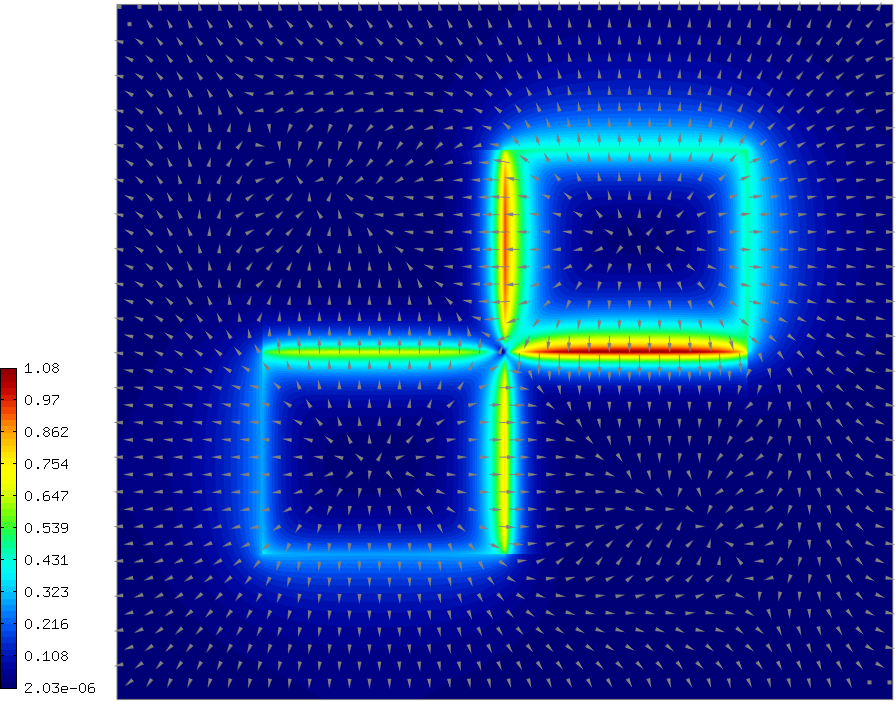
\includegraphics[width=.4\textwidth]{saphir/flux1.png}
}\\[.5em]
\subfigure[$\phi^2_s$]{
  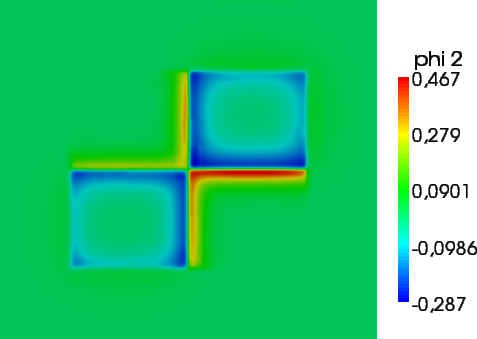
\includegraphics[width=.44\textwidth]{saphir/flux2p.png}
}
\hspace{1em}
\subfigure[$\phi_3^s$]{
  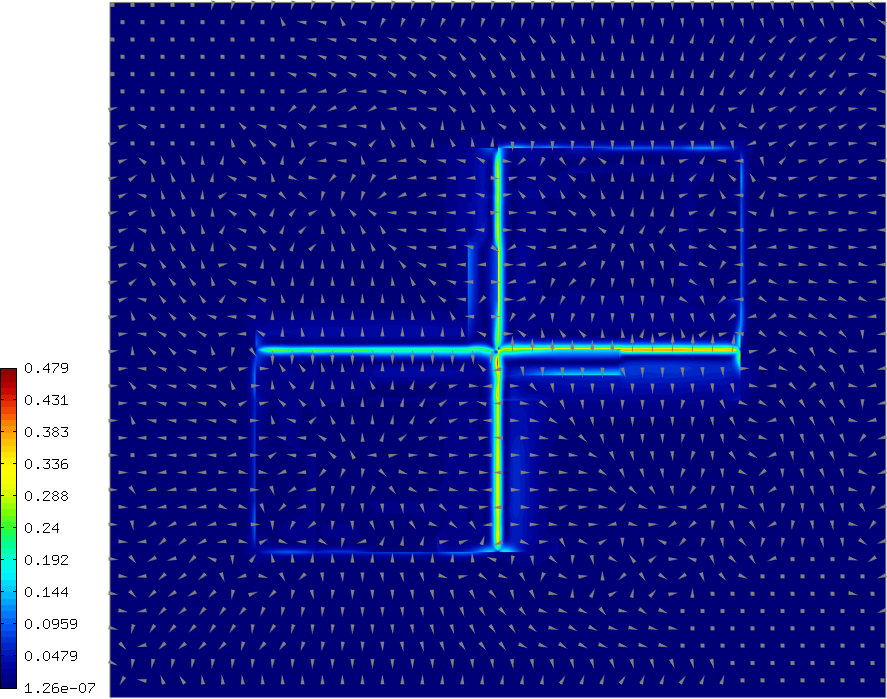
\includegraphics[width=.4\textwidth]{saphir/flux3.png}
}\\[.5em]
%\caption[Solution of the IAEA EIR-1 benchmark (\text{SP}_5)]{Solution of the IAEA EIR-1 benchmark
 %  (\SPN[5] approximation). Even order moments visualized using Paraview, odd order moments using Hermes2D internal
 %  capabilities.}
 %\label{fig:41}
%\end{figure}
%
%\begin{figure}[!ht]
%\ContinuedFloat
%\centering
\subfigure[$\phi^4_s$]{
  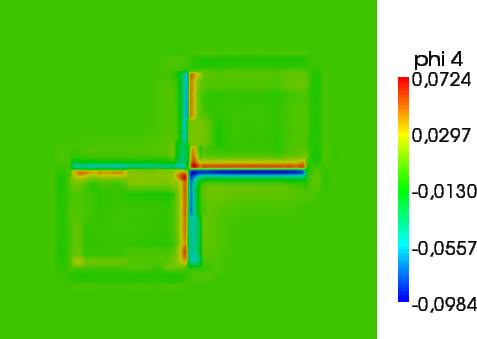
\includegraphics[width=.44\textwidth]{saphir/flux4p.png}
}
\hspace{1em}
\subfigure[$\phi_5^s$]{
  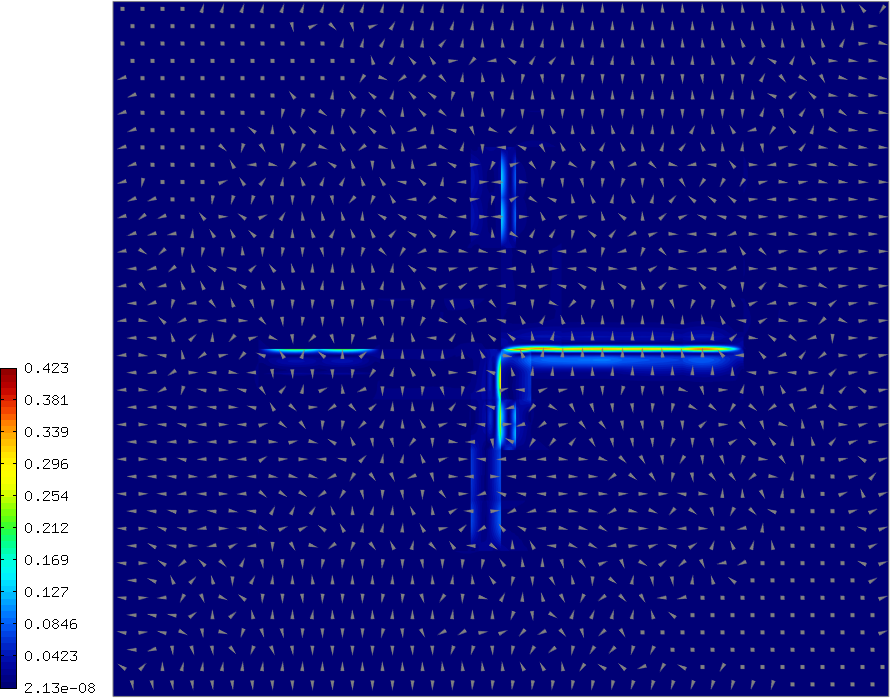
\includegraphics[width=.4\textwidth]{saphir/flux5.png}
}
\caption[Solution of the IAEA EIR-1 benchmark ($\text{SP}_5$)]{Solution of the IAEA EIR-1 benchmark
   (\SPN[5] approximation). Even order moments visualized using Paraview, odd order moments using Hermes2D internal
   capabilities.}
  \label{fig:41}
\end{figure}

\begin{figure}[!hb]
\centering
\subfigure[$\phi$]{
  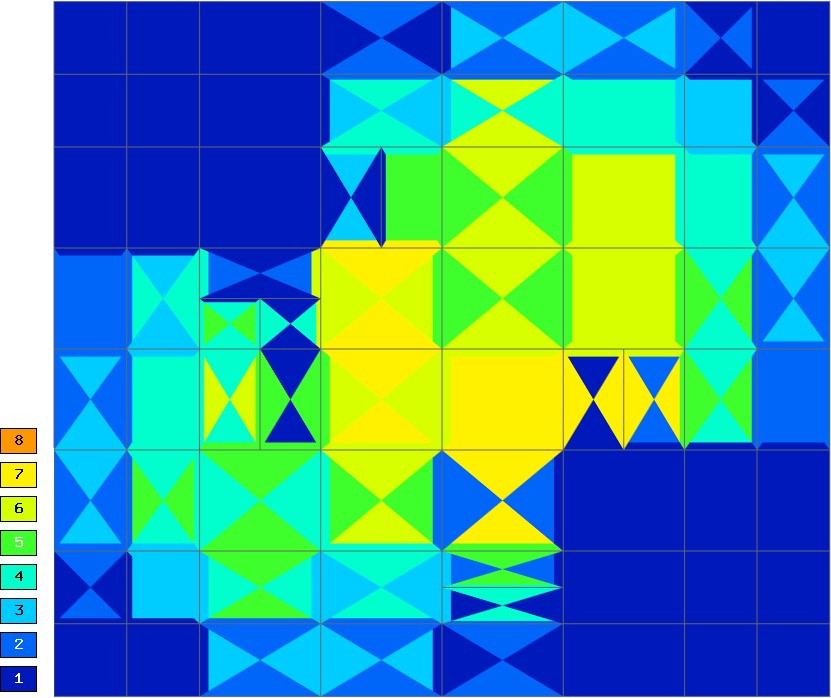
\includegraphics[width=.32\textwidth]{saphir/mesh0.png}
}
\hspace{1em}
\subfigure[$\phi_2^s$]{
  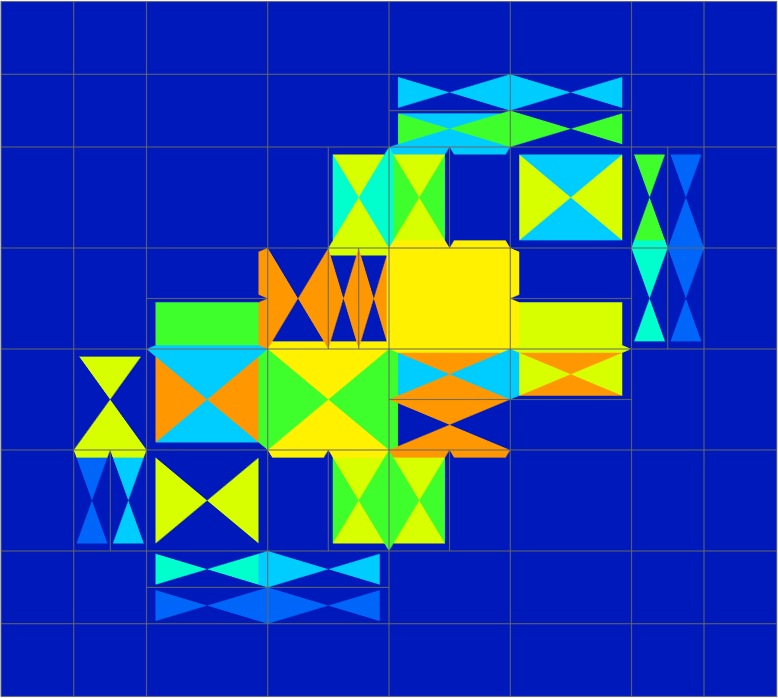
\includegraphics[width=.3\textwidth]{saphir/mesh2.png}
}\\[.5em]
\subfigure[$\phi^4_s$]{
  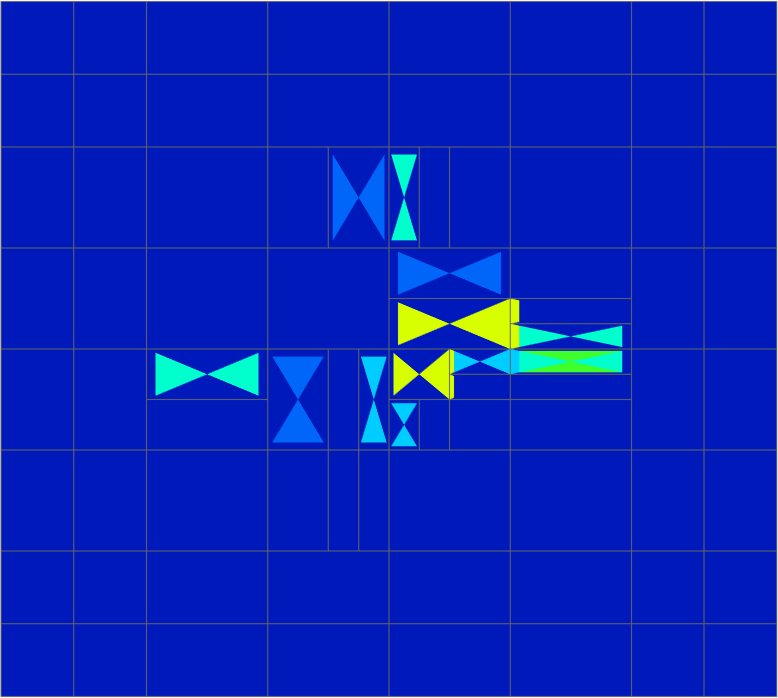
\includegraphics[width=.3\textwidth]{saphir/mesh4.png}
}
\caption[Approximation spaces for the IAEA EIR-1 benchmark ($\text{SP}_5$)]{Approximation spaces for the IAEA EIR-1
benchmark (\SPN[5] approximation).}
  \label{fig:43}
\end{figure}

Figures \ref{fig:41} show the shape of the $\SPN[5]$ solution. It consists of the scalar
flux and the even-order moments $\phi^s_2$, $\phi^s_4$ ($\SPN$ fluxes) as well as the odd-order vector moments ($\SPN$
currents) obtained from the even order moments by eq. \eqref{eq:spncur} (with derivative replaced by gradient).
Notice the decreasing magnitude of the higher-order moments -- the shape of the scalar flux is largely determined by the
zero-th $\SPN[5]$ moment $\phi^s_0$, while the higher-order moments provide transport corrections mostly visible at the region interfaces. Also note from \eqref{eq:SPN_scalar_flux} that the contributions of the higher-order moments to the scalar
flux are further weighted by less than 1 factors. Nevertheless, even these small corrections can have important impact
on the overall results, as shown in \ref{tab:IAEA}, where average scalar fluxes in regions 1 to 5 are compared with the
$\SN[8]$ results reported by \cite{Coppa1}. Note that relatively large homogeneous regions in this example (typical for
whole-core reactor calculations) make it fit well into the asymptotic region of validity of the $\SPN$ approximation.

\begin{table}
\centering
\begin{tabular}{c|cccc}
		Region \# & $\SPN[1]$ & $\SPN[3]$ & $\SPN[5]$ & $\SPN[7]$ \\\hline
		1   & 0.81 & 0.12 & 0.06 & 0.05 \\[.2em] 
		2   & 5.23 & 0.80 & 0.31 & 0.26 \\[.2em] 
		3   & 0.90 & 0.14 & 0.07 & 0.07 \\[.2em] 
		4   & 3.86 & 0.61 & 0.39 & 0.37 \\[.2em] 
		5   & 0.84 & 0.06 & 0.06 & 0.08 \\[.2em]\hline
		$t_{\mbox{\scriptsize CPU}}$ [s] & 4.1 & 16.7 & 42.5 & 66.7  
	\end{tabular} 
\caption[$\text{SP}_{5}$ vs. $\text{S}_{8}$ on the IAEA EIR-1 benchmark] {Rel. errors [\%] of average scalar flux in
regions $i=1,\ldots,5$ w.r.t. $S_8$}
\label{tab:IAEA}
\end{table}

The solution was spatially converged using the $hp$-adaptivity of Hermes2D with convergence criterion
$\norm[1]{\Ehp^{\phi}} < 0.5\%$ (chosen as a reasonable value from the engineering point of view). Figure \fref{fig:42}
shows the convergence curves for the $\SPN$ fluxes (labeled ``pseudo-fluxes'' in the figure), scalar fluxes and the
region-average scalar fluxes. Note how the scalar flux error estimate stays closely below the combined estimate of the
$\SPN$ fluxes error, verifying \eqref{eq:err-est-phi}.

\begin{figure}[!ht]
\centering
  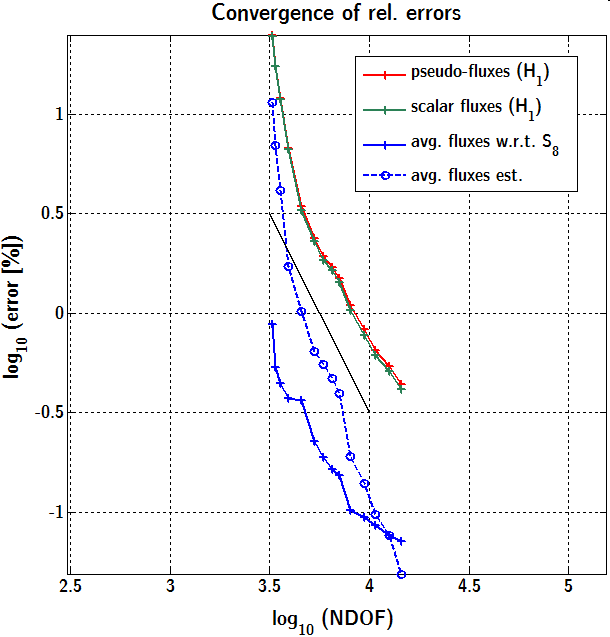
\includegraphics[scale=.5]{saphir/conv_dof_sp5}
  \caption[Adaptivity convergence curves for the IAEA EIR-1 benchmark]{Adaptivity convergence curves for the 
  IAEA EIR-1 benchmark (black line corresponds to fourth-order convergence) -- $\text{SP}_5$ approximation}
  \label{fig:42}
\end{figure}

Figure \ref{fig:43} shows the distribution of final mesh sizes and local approximation orders and emphasize
the utility of multimesh approximation and anisotropic adaptivity. 
As a legend for these and later approximation order
figures, consider the element in \fref{fig:44}.
\begin{figure}[!ht]
\centering
  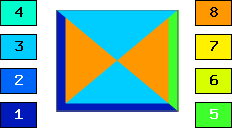
\includegraphics[scale=.6]{elem}
  \caption[Legend for the approximation order figures]{Legend for the approximation order figures.}
  \label{fig:44}
\end{figure}
The colors encode that a tensor product of 1D polynomials of degree up to 3 and 8 in the horizontal and vertical
direction, respectively, is used to define the local approximation space for this element. Edge shape functions are
constrained by edge shape functions of the adjacent elements, so as to satisfy the $H^1$ conformity constraints 
(\cite[\S3.5.5]{Hermes-book1}).



\subsubsection{The $7\times 7$ PWR assembly example (Stankovski benchmark)}\label{sec:stankovski}

This example from \cite[Sec. 6.4.2]{dragon} represents a one-group calculation of neutron flux distribution in a
small-scale model of a typical pressurized water reactor fuel assembly.
\begin{figure}[!ht]
\centering
  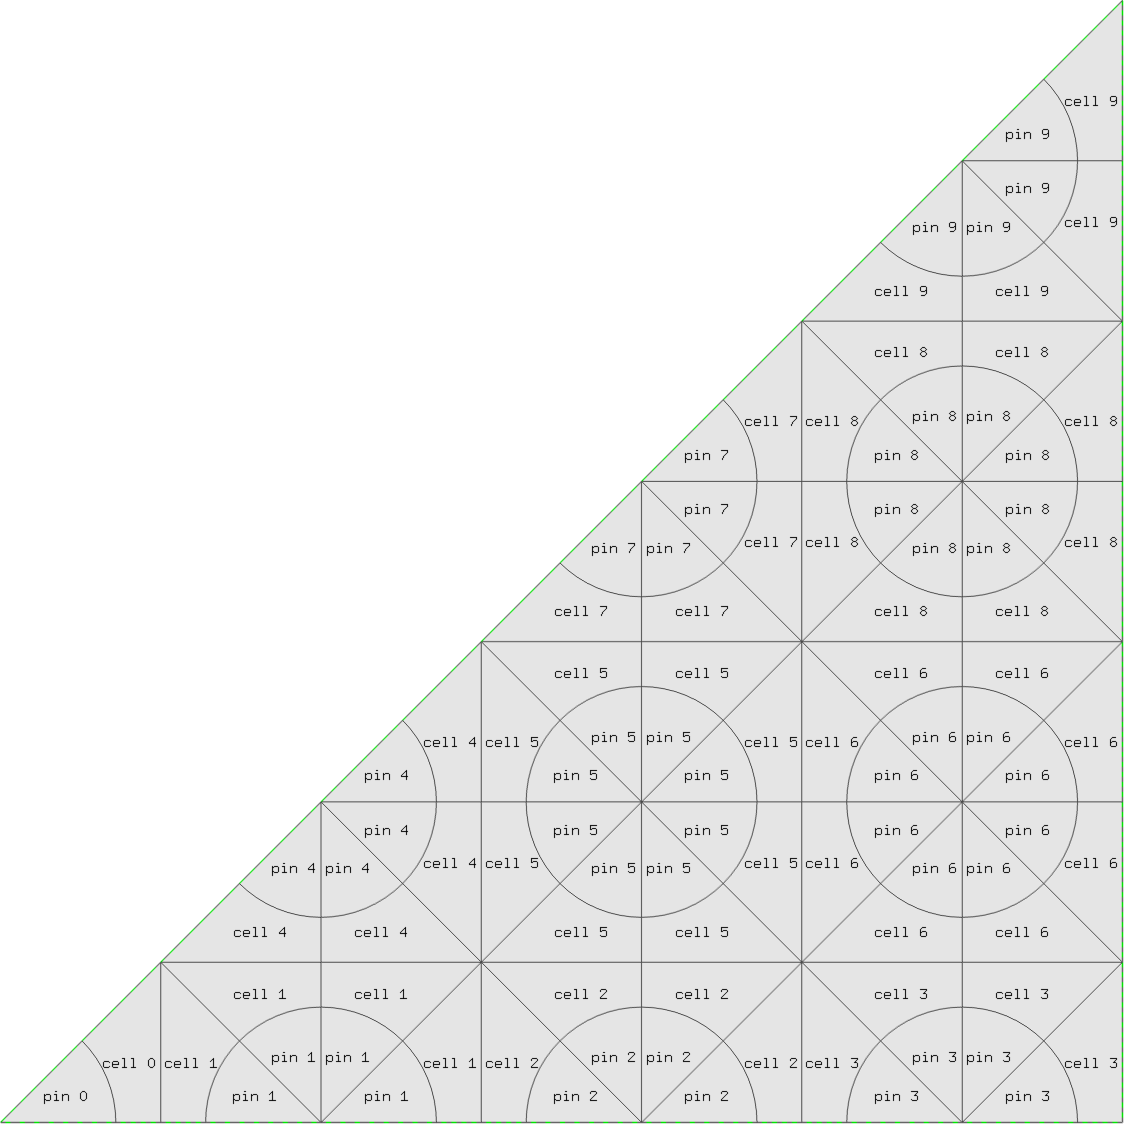
\includegraphics[width=.5\textwidth]{stankov/meshh}
  \caption[Geometry of the Stankovski benchmark]{Geometry of the Stankovski benchmark.}
  \label{fig:30}
\end{figure}
 The isotropic fixed source of
\SI{1.0}{cm^{-3}.sec} is specified in all regions marked as \texttt{cell\#} in \fref{fig:30} so as to represent neutrons
scattered into the first group during their slowing-down in the moderator regions. Each moderator region has $\sigma_t
= \SI{1.250}{cm^{-1}}$, $\sigma_s = \SI{1.242}{cm^{-1}}$, while each fuel region marked as \texttt{pin\#} in
\fref{fig:30} with the exception of \texttt{pin0} has $\sigma_t = \SI{0.625}{cm^{-1}}$, $\sigma_s =
\SI{0.355}{cm^{-1}}$. Purely absorbing region \texttt{pin0} with $\sigma_t =
\SI{14}{cm^{-1}}$ corresponds to a control rod. The width of each square cell is \SI{0.45}{cm} and fuel pin radius is
\SI{0.45}{cm} and vacuum boundary is assumed at the right side while reflective boundary at the remaining sides. The
ability of Hermes2D to use finite elements with curved boundaries with known non-uniform rational B-spline (NURBS) parametrization \cite{Hermes-book1} has been utilized to treat the circular fuel pin boundary exactly.
\begin{figure}[!ht]
\centering
  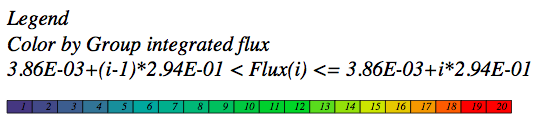
\includegraphics[scale=.4]{stankov/DRAGONl}\\
  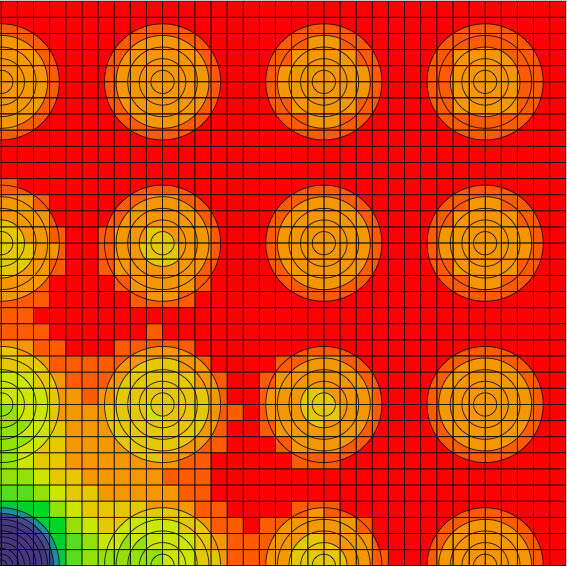
\includegraphics[scale=.4]{stankov/DRAGON}
  \caption[Stankovski benchmark -- reference solution by DRAGON]{Stankovski benchmark -- reference solution by DRAGON
  (method of characteristics, 2048 regions, quadrature order 20, integration lines spacing \SI{100}{cm^{-1}}); only a
  first quadrant is shown (extends by reflectional symmetry). Values span the range $[3.86\times 10^{-3},
  5.88386]$.}
  \label{fig:39}
\end{figure}

\begin{figure}[!ht]
\centering
\subfigure[$\phi$]{
  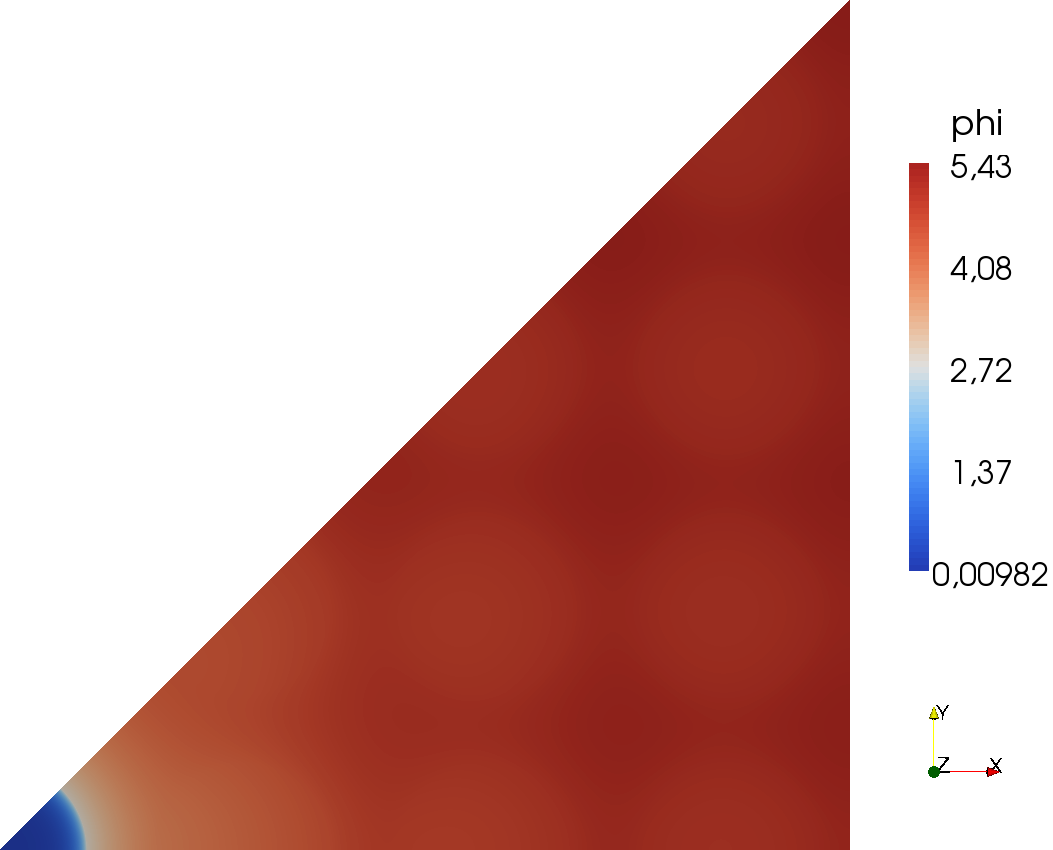
\includegraphics[scale=.18]{stankov/SP3_0.png}
}
\hspace{.1em}
\subfigure[$\phi^s_2$]{
  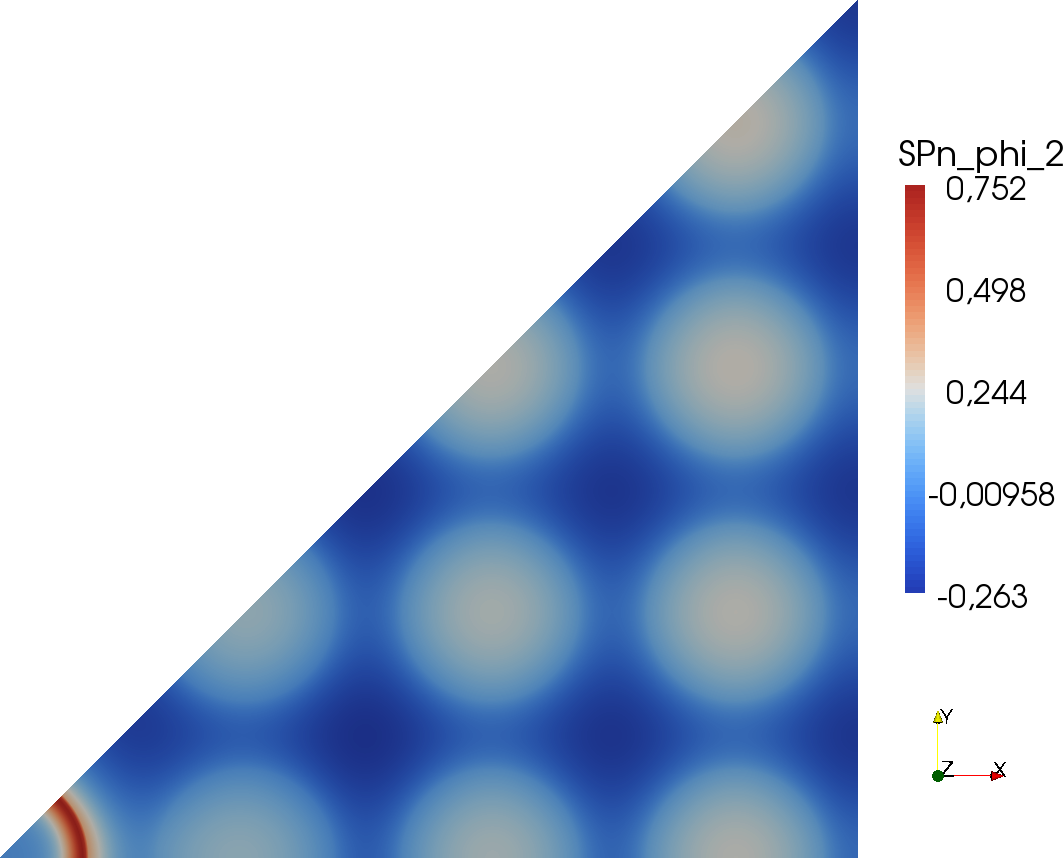
\includegraphics[scale=.18]{stankov/SP3_2.png}
}
  \caption[Solution of the Stankovski benchmark ($\text{SP}_3$)]{Solution of the Stankovski benchmark
  (\SPN[3]).}
  \label{fig:33}
\end{figure}
\begin{figure}[!ht]
\centering
\subfigure[$\phi^s_0$]{
  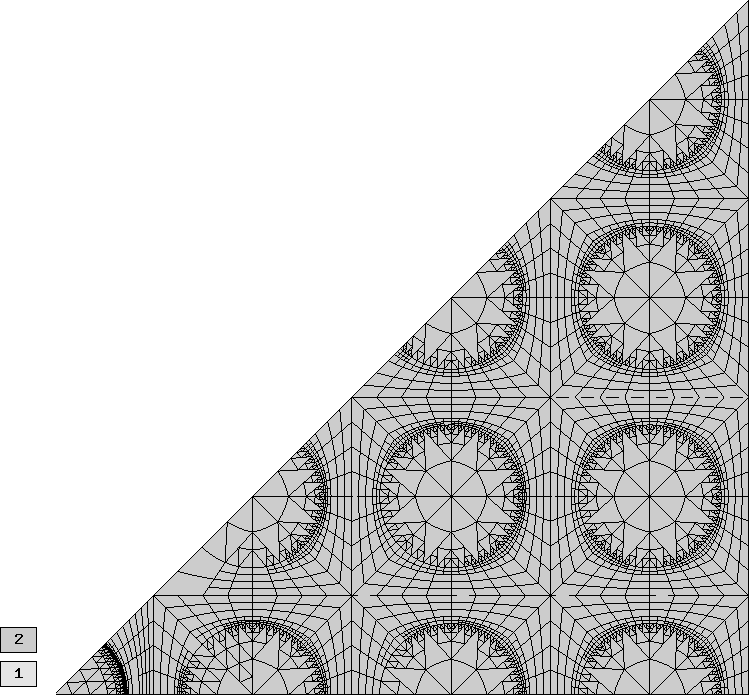
\includegraphics[scale=.22]{stankov/mesh0.png}
}
\hspace{3em}
\subfigure[$\phi^s_2$]{
  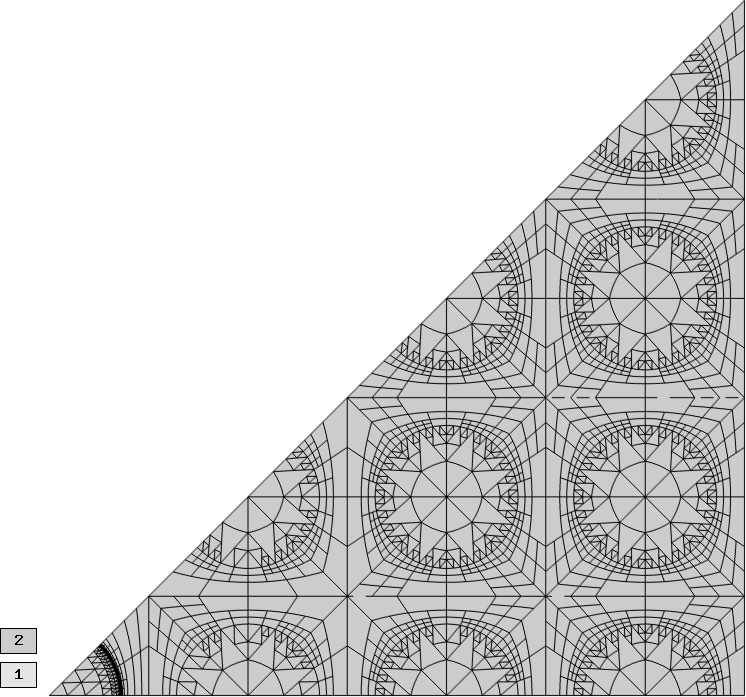
\includegraphics[scale=.22]{stankov/mesh2.png}
}
  \caption[Approximation spaces in the Stankovski benchmark ($\text{SP}_3$)]{Approximation spaces for the Stankovski
  benchmark (\SPN[3]).}
  \label{fig:36}
\end{figure}

Figures \ref{fig:33} and \ref{fig:36} show the $\SPN[3]$ solution with the underlying meshes obtained from the simple
$h$-adaptivity based on the error estimate of Kelly et al. as outlined in the last paragraph of \sref{sec:hermes_adapt}.
For comparison,
the $\SPN[1]$ (diffusion), $\SPN[5]$ and $\SN[8]$ solutions are also shown in figures \ref{fig:32}, \ref{fig:37} and 
\ref{fig:38}, respectively.
Note that scalar flux is displayed instead of $\phi_0^s$ in the $\SPN$ figures
to facilitate the comparison.



\begin{figure}[!ht]
\centering
  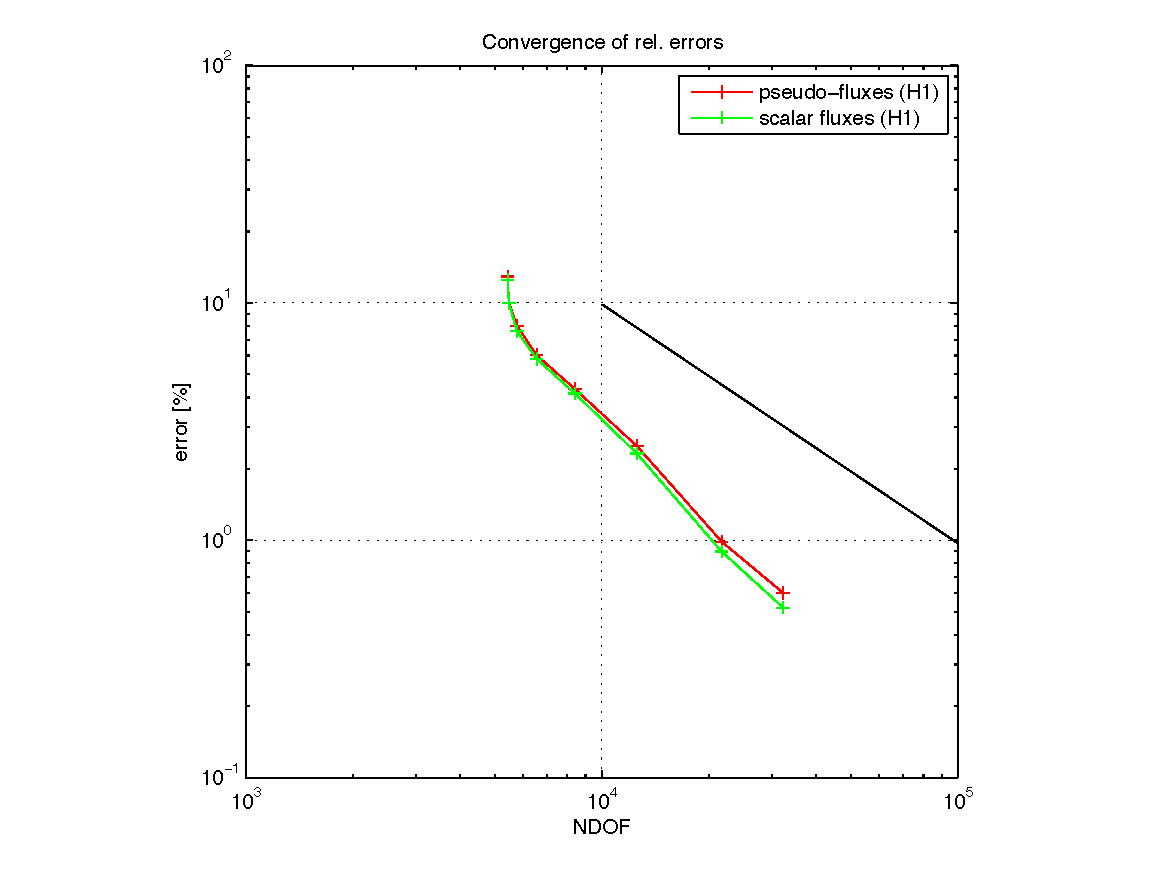
\includegraphics[scale=.45]{stankov/conv_dof_sp5}
  \caption[Adaptivity convergence curves for the Stankovski benchmark ]{Adaptivity convergence curves for the 
  Stankovski benchmark (black line corresponds to second-order convergence) -- $\text{SP}_5$ approximation,
  bi-quadratic finite elements.}
  \label{fig:39}
\end{figure}


\begin{figure}[!ht]
\centering
  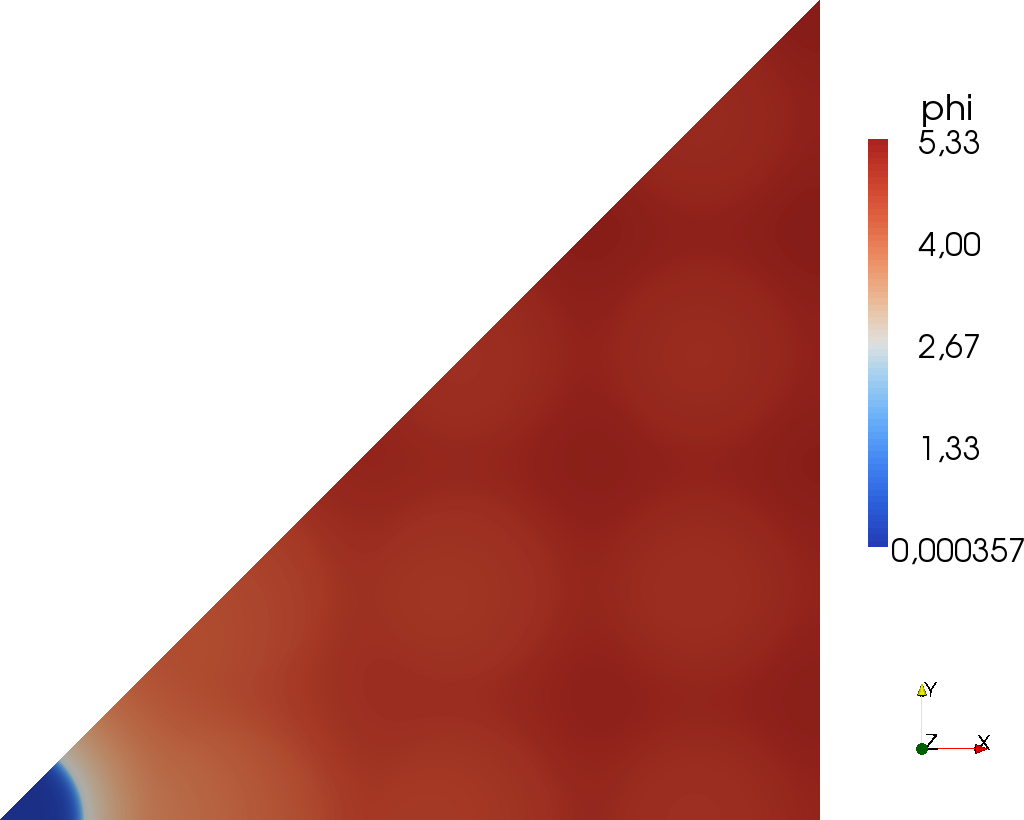
\includegraphics[scale=.17]{stankov/SP1.png}
  \caption[Solution of the Stankovski benchmark ($\text{SP}_1$)]{Solution of the Stankovski benchmark
   (\SPN[1]).}
  \label{fig:32}
\end{figure}
\begin{figure}[!ht]
\centering
\subfigure[$\phi$]{
  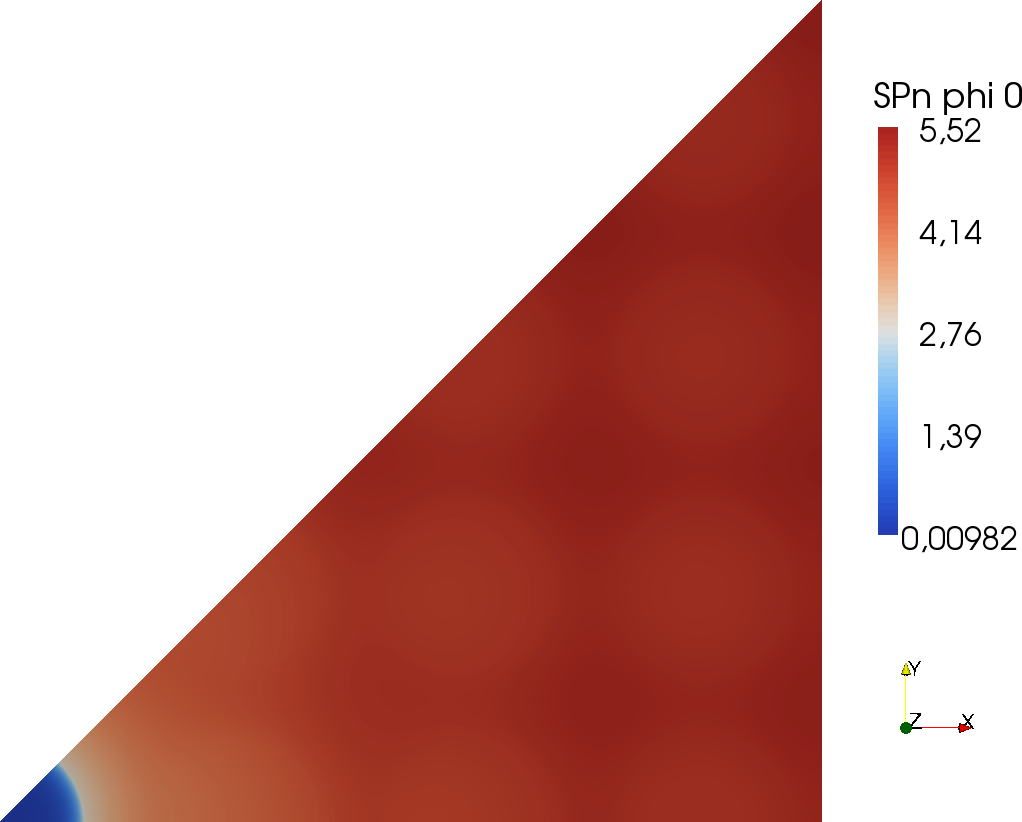
\includegraphics[scale=.17]{stankov/SP5_0.png}
}
\hspace{.1em}
\subfigure[$\phi_2^s$]{
  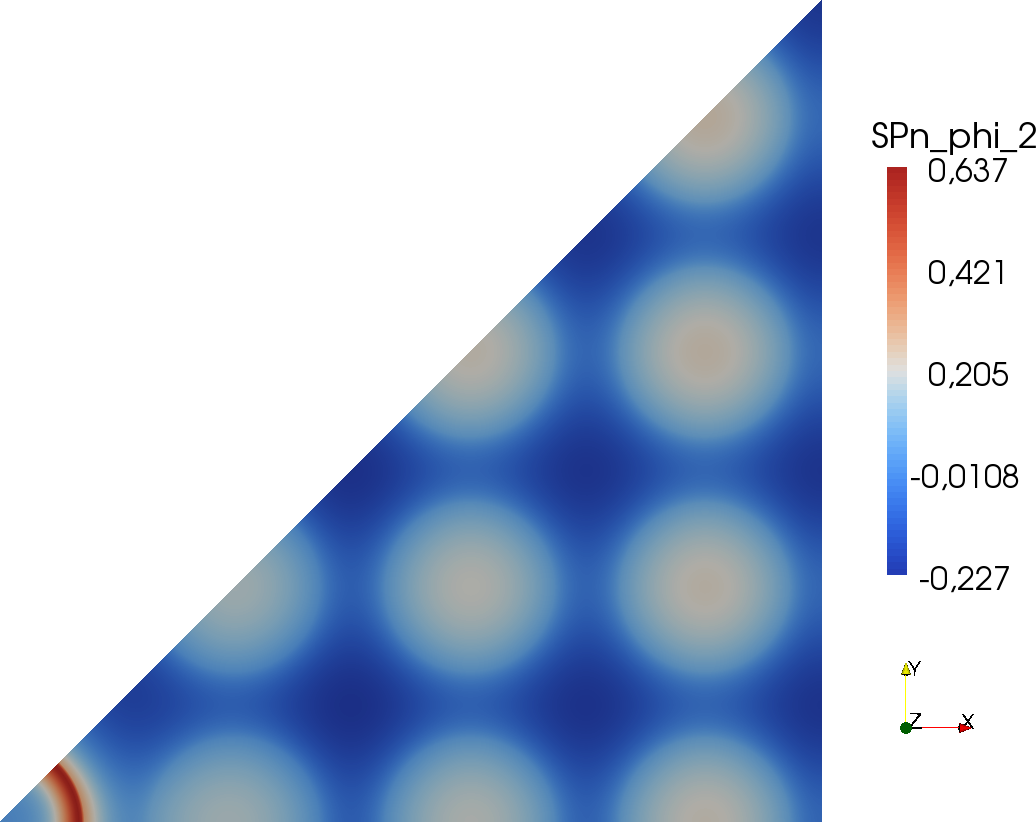
\includegraphics[scale=.17]{stankov/SP5_2.png}
}
\\
\subfigure[$\phi^4_s$]{
  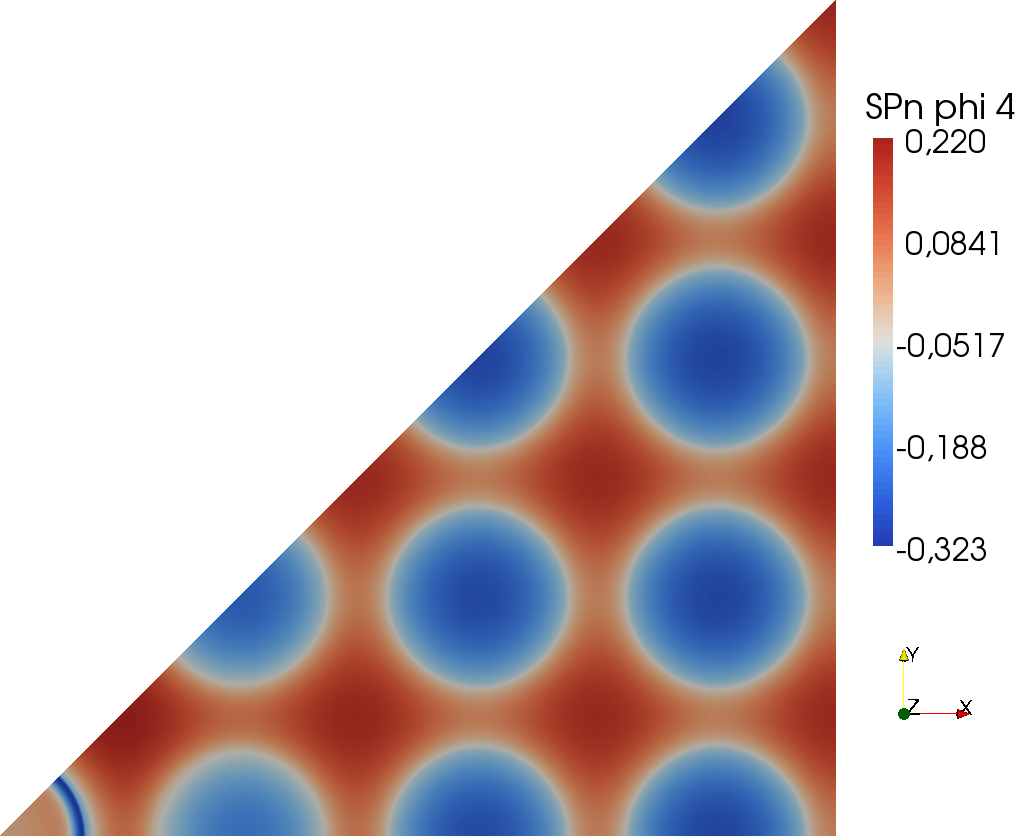
\includegraphics[scale=.17]{stankov/SP5_4.png}
}
  \caption[Solution of the Stankovski benchmark ($\text{SP}_5$)]{Solution of the Stankovski benchmark
   (\SPN[5]).}
  \label{fig:37}
\end{figure}
\begin{figure}[!ht]
\centering
  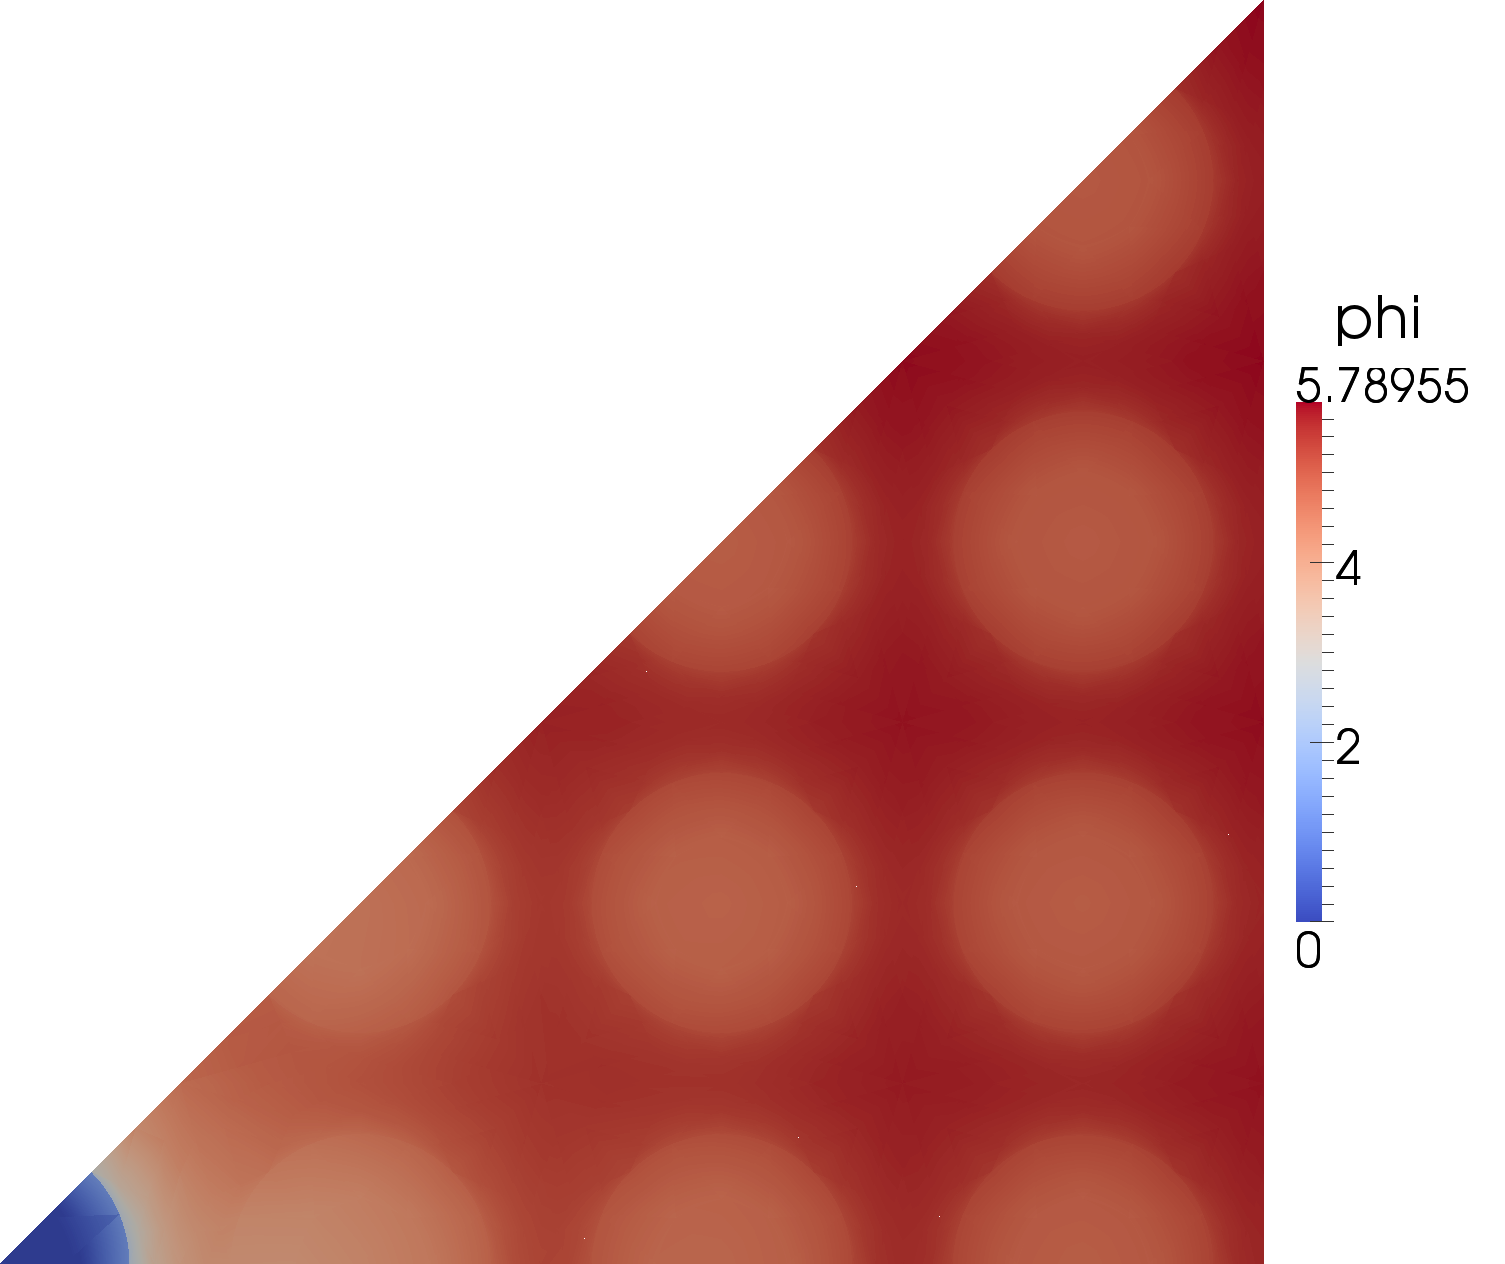
\includegraphics[scale=.11]{stankov/s8.png}
  \caption[Solution of the Stankovski benchmark ($\text{S}_8$)]{Solution of the Stankovski benchmark
   (\SN[8]).}
  \label{fig:38}
\end{figure}

These figures show the effort of the higher-order $\SPN$
approximations to recover the strong gradient of scalar flux at the fuel pin boundaries via the $\SPN$ fluxes $\phi^s$
(serving as correcting terms in \eqref{eq:SPN_scalar_flux}). The comparison of absorption rates
$$
	\int_{V_i} \sigma_{a,i} \phi(\br)\,\d{\br},\quad i = 1,2,\ldots,20,
$$
where $V_i$ corresponds subsequently to \texttt{pin0}, \texttt{cell0}, \texttt{pin1}, \texttt{cell1}, etc., with the
reference solution obtained from DRAGON (\fref{fig:39}) indicates the limitation of the $\SPN$ approximations
when used outside their asymptotic range of theoretical validity (note that in some regions, the $\SPN[5]$ errors are even slightly bigger than the
$\SPN[3]$ errors). We note that maximal difference between the reference region-wise integrated absorption rates and
those obtained from the $\SN[8]$ method implemented in Hermes2D was only 0.313\% (more $\SN$ examples in Hermes2D will
be presented in \sref{sec:snex}).


 
\subsubsection{One-group hexagonal eigenvalue example}
This example has been proposed in \cite{hebert} to test the mixed finite element discretization of the $\SPN$ equations.
\begin{table}[!ht]
\centering
\begin{tabular}{c|cccc}
Region \# & $\sigma_t\ [\SI{}{cm^{-1}}]$ & $\sigma_{s0}\ [\SI{}{cm^{-1}}]$ & $\sigma_{s1}\ [\SI{}{cm^{-1}}]$ &
$\nu \sigma_{f}\ [\SI{}{cm^{-1}}]$ \\\hline 
		1   & 0.025 & 0.013 & 0.0   & 0.0155\\[.2em] 
		2   & 0.025 & 0.024 & 0.006 & 0.0 \\[.2em] 
		3   & 0.075 & 0.0 & 0.0     & 0.0
\end{tabular}
\caption[Material properties of the 1-group eigenvalue example]{Material properties of the 1-group eigenvalue example.}
\label{tab:prop5}
\end{table}
It represents a criticality eigenvalue problem with anisotropic scattering.

\begin{figure}[!ht]
\centering
  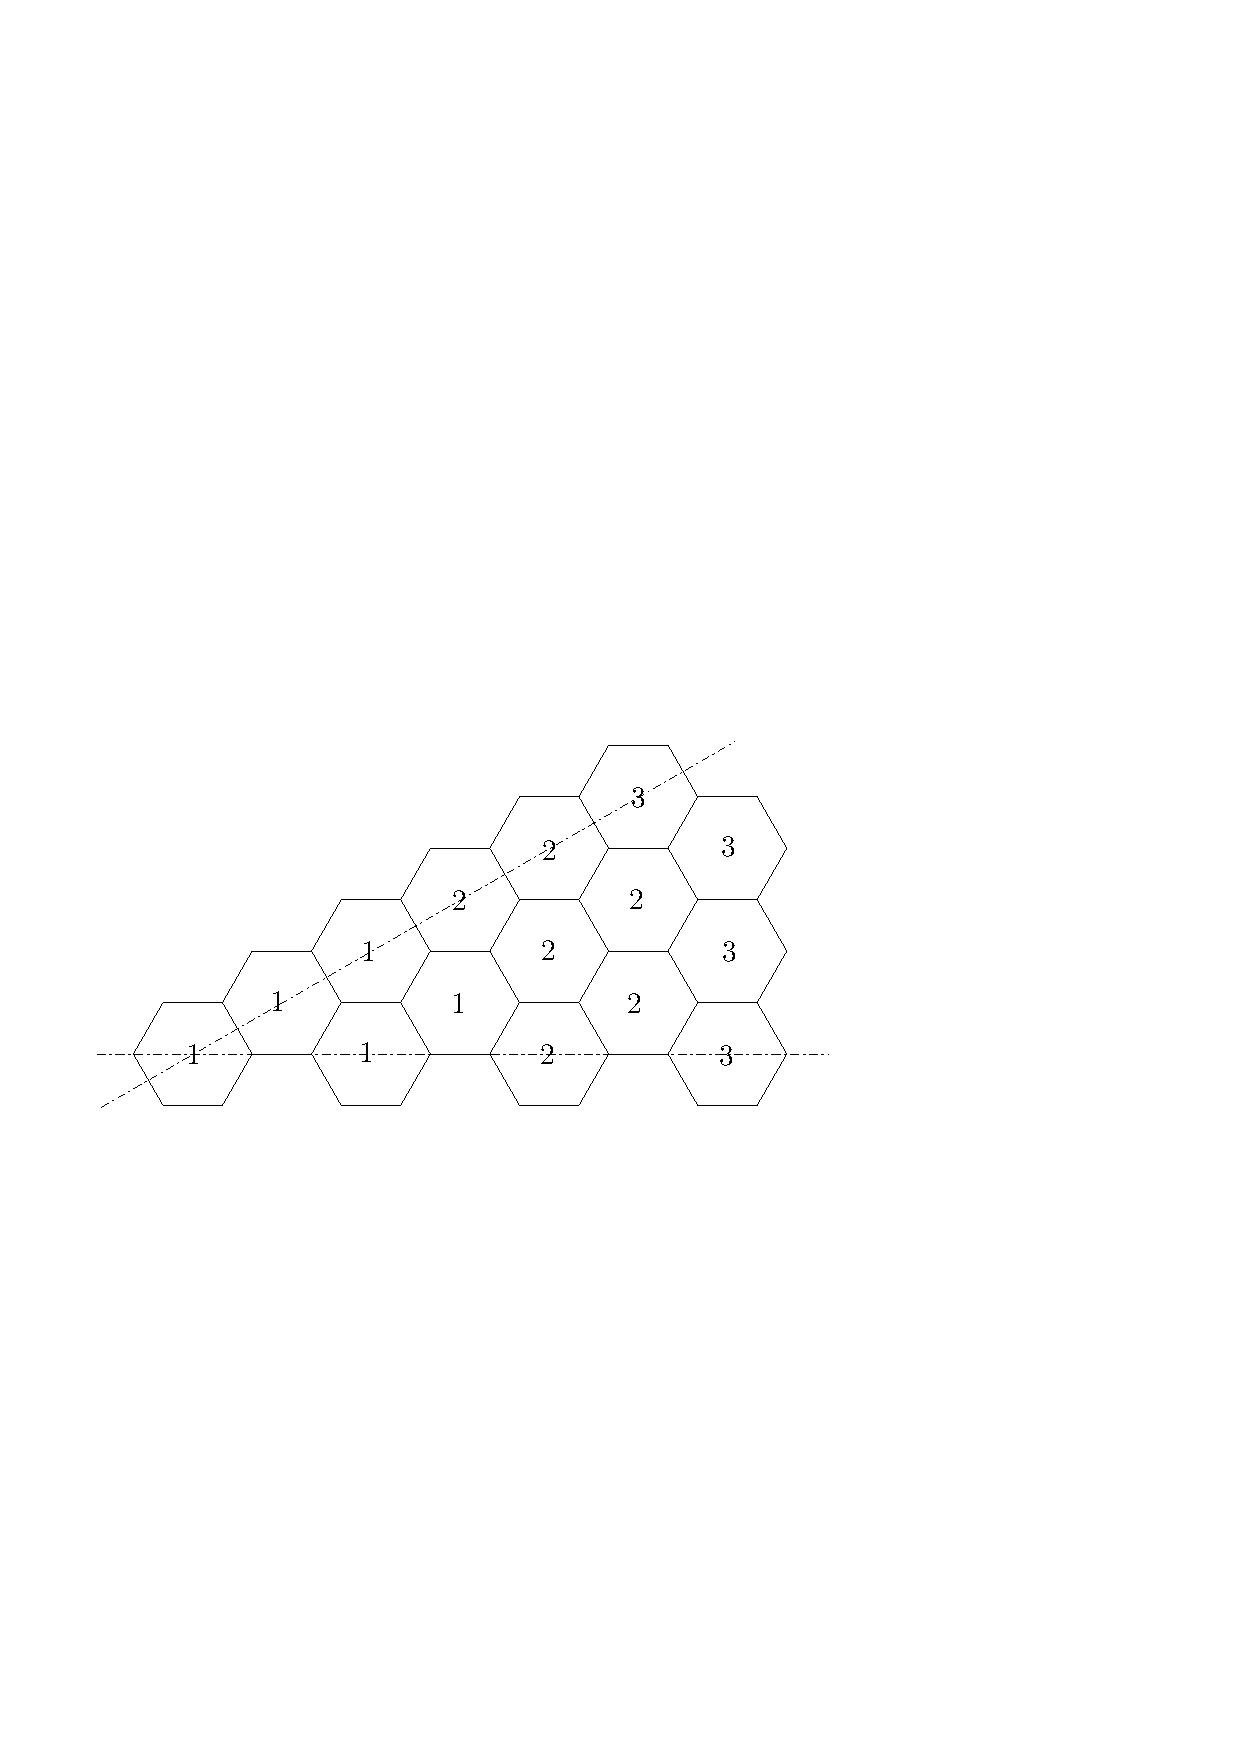
\includegraphics[scale=.55]{hex/def}
  \caption[Geometry of the 1-group eigenvalue example]{Geometry of the 1-group eigenvalue example. Each hexagonal
  assembly has side length \SI{19}{cm}.
  Vacuum boundary conditions at the right boundary, reflective conditions along the dash-dotted lines.}
  \label{fig:50}
\end{figure} 

\begin{figure}[!ht]
\centering
  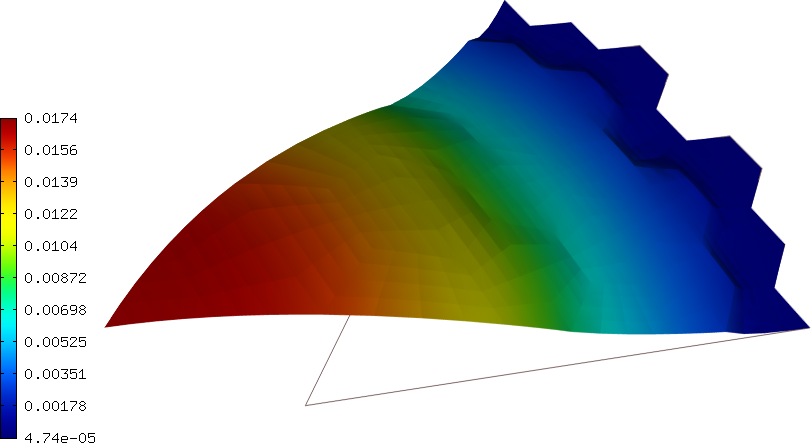
\includegraphics[scale=.25]{hex/f0.png}
	\hspace{.5em}
  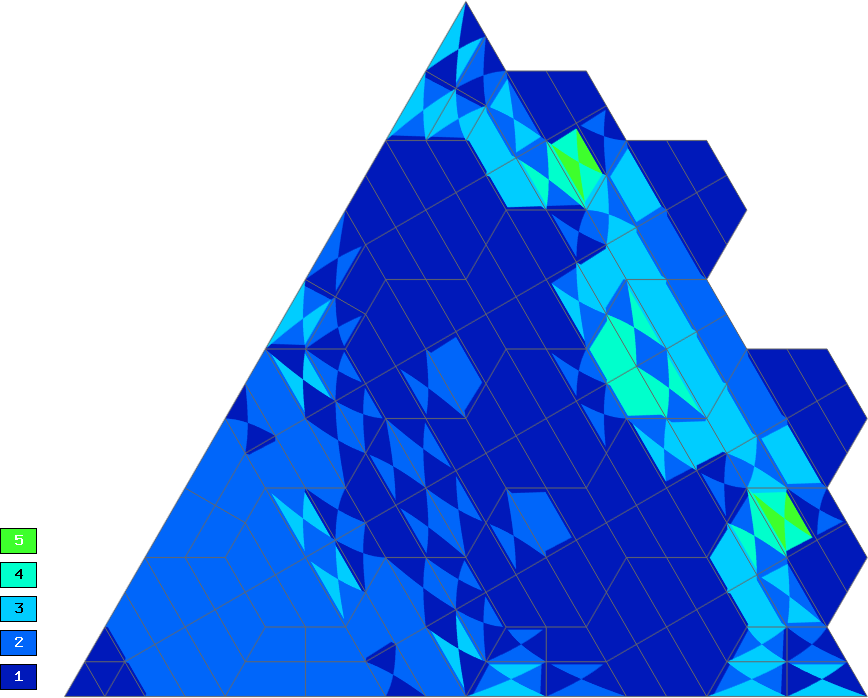
\includegraphics[scale=.19]{hex/mesh_f0.png}
	\caption[Solution of the 1-group eigenvalue example]{1-group eigenvalue example -- $\phi_0^s$.}
	\label{fig:51}
\end{figure}
\begin{figure}[!ht]
\centering
  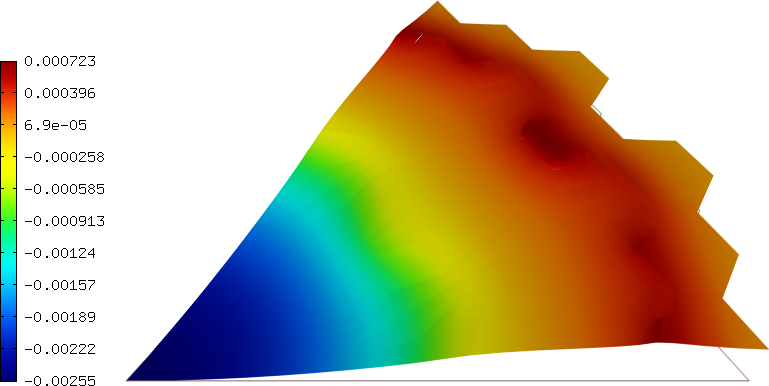
\includegraphics[scale=.25]{hex/f2.png}
	\hspace{.5em}
  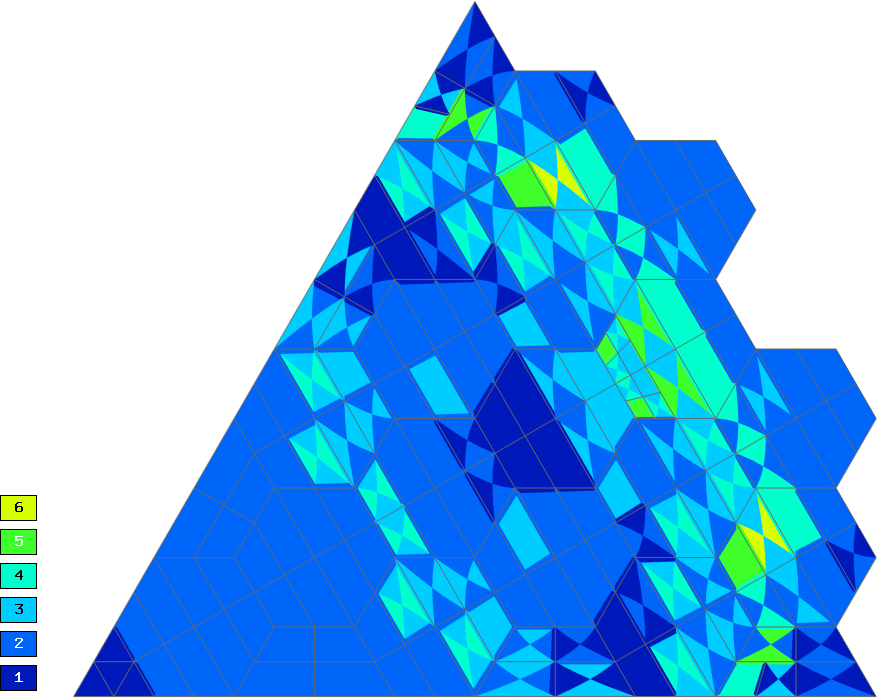
\includegraphics[scale=.19]{hex/mesh_f2.png}
	\caption[Solution of the 1-group eigenvalue example]{1-group eigenvalue example -- $\phi_2^s$.}
	\label{fig:52}
\end{figure}
\begin{figure}[!ht]
\centering
  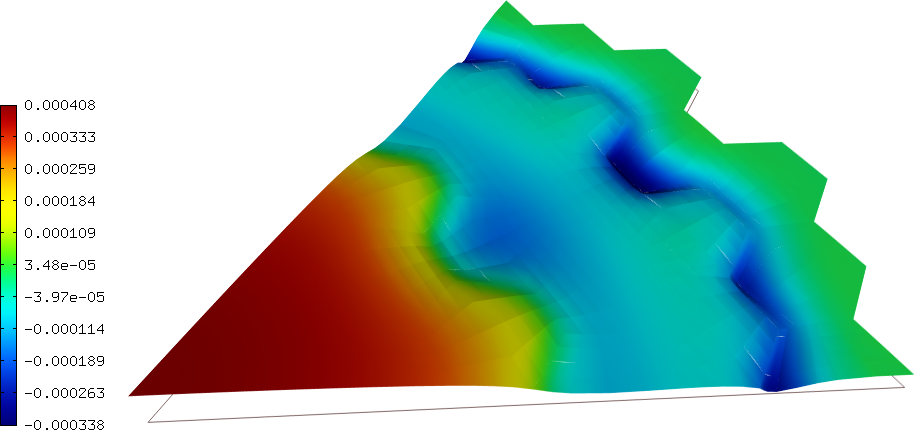
\includegraphics[scale=.25]{hex/f4.png}
	\hspace{.5em}
  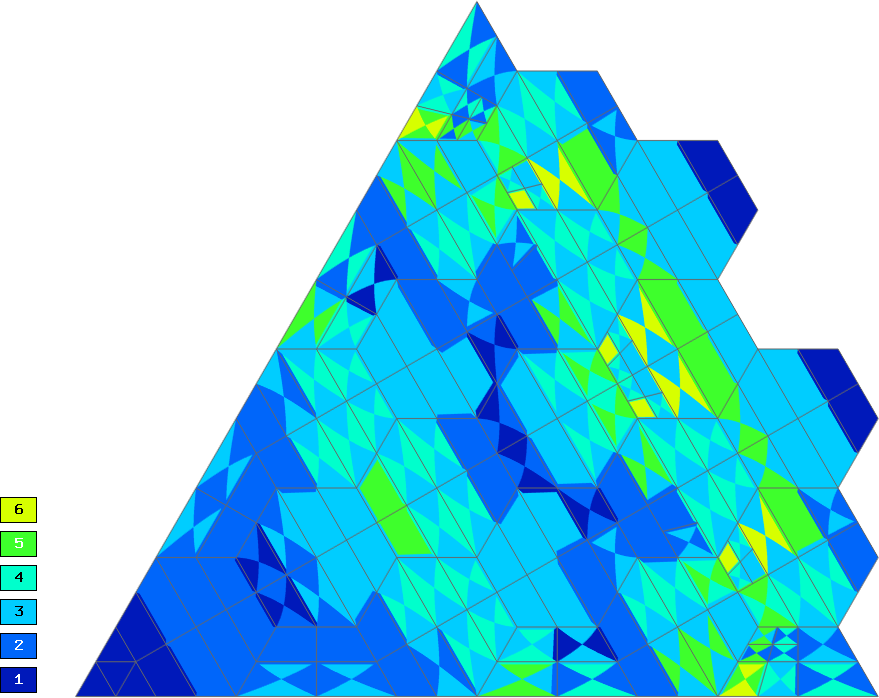
\includegraphics[scale=.19]{hex/mesh_f4.png}
	\caption[Solution of the 1-group eigenvalue example]{1-group eigenvalue example -- $\phi_4^s$.}
	\label{fig:53}
\end{figure}

Figures \ref{fig:51} to \ref{fig:53} show
the $\SPN[5]$ solution (even order $\SPN[5]$ fluxes) and the corresponding distribution of approximation orders and mesh
sizes. At each adaptivity step, the Rayleigh-quotient iteration has been used to obtain the reference solution on the
globally refined spaces, starting from orthogonal projection of the solution from previous 
adaptivity step onto these spaces (unit constant function has been used as initial shape of all moments). A decreasing
tolerance has been used for the eigenvalue iteration, starting with $10^{-3}$ and decreasing all the way down to
$10^{-10}$ by multiplication with $0.1$ at each adaptivity step (the actual residual norm ratio to the initial one has
been used to measure convergence:
$$\frac{(\norm{\mat{A} - \lambda^{(i)}\mat{B})\mat{x}^{(i)}}}{(\norm{\mat{A} - \lambda^{(0)}\mat{B})\mat{x}^{(0)}}},
$$
where $\lambda^{(k)}$ is obtained from the Rayleigh quotient with $\mat{x}^{(k)}$).

\begin{figure}[!ht]
\centering
  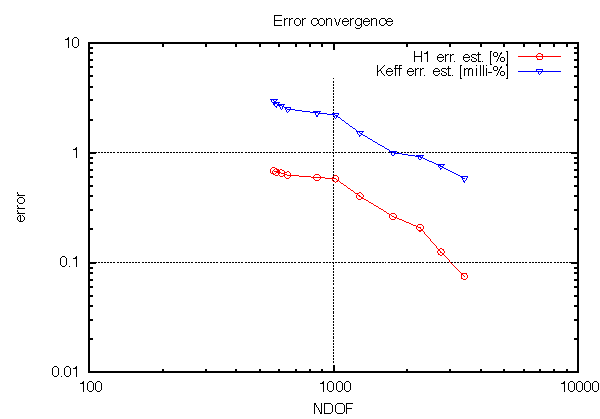
\includegraphics[scale=1.1]{hex/conv_dof}
  \caption[Adaptivity convergence curves for the 1-group eigenvalue example]{Adaptivity convergence curves for the
  1-group eigenvalue example. The reference value $\keff = 1.001271$ provided by \cite{hebert}.}
  \label{fig:57}
\end{figure}

\begin{figure}[!hb]
\centering
  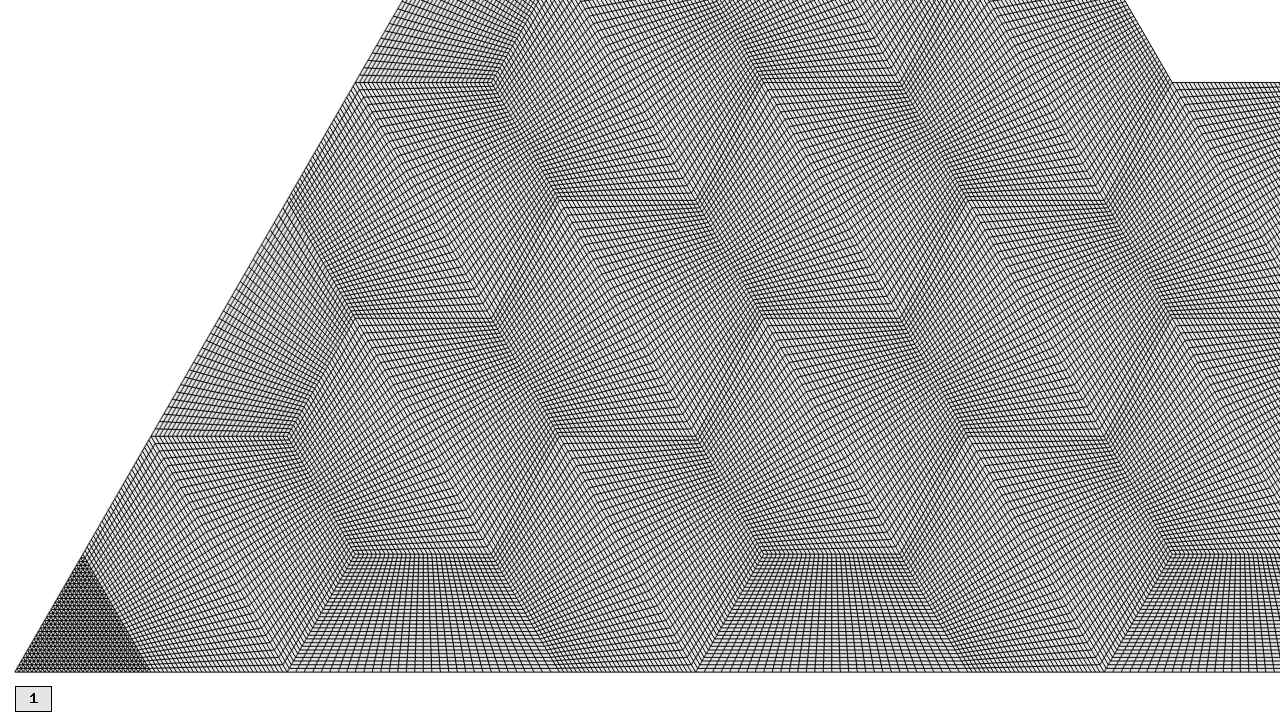
\includegraphics[scale=.33]{hex/ref.png}
	\caption[1-group eigenvalue example (uniformly refined mesh)]{1-group eigenvalue example (uniformly refined mesh).}
	\label{fig:58}
\end{figure}

The error in the final eigenvalue with respect to the reference solution from \cite{hebert} was less than one
milli-percent (pcm) as can be seen from the convergence curve in \fref{fig:57} (exactly \SI{0.5813}{pcm}) and the
adaptivity convergence criterion \mbox{$\norm[1]{\Ehp^{\phi}} < 0.1\%$} was reached in 40.5 seconds. For comparison,
using piecewise linear finite element approximation on the globally heavily refined mesh (\fref{fig:58}) resulted in the eigenvalue difference of \SI{2.78470}{pcm} in 378.1 seconds (still using the direct solver UMFPACK with the same settings).
Note that the reference solution in \cite{hebert} was obtained using an approximation space with 118677 degrees of
freedom, while the finest globally-refined space needed to obtain the solutions depicted in the figures in this section
using the $hp$-adaptivity in Hermes2D had 31898 degrees of freedom.

%\clearpage
\subsubsection{Two-group WWER-440 criticality benchmark (diffusion)}
This benchmark has been defined in \cite{Chao2} to test nodal diffusion method against fine-mesh finite-difference
solution of a two-group criticality eigenvalue problem for a core of the WWER-440 reactor with 1/12th reflectional
symmetry.
In the WWER-440 reactor, the control rods are represented by whole assemblies that push the regular fuel
assemblies out of the core and replace their position. As a consequence, the multiplying medium with fission
sources gets replaced by highly absorbing medium with no source, leading to strong solution gradients at the interface
between the control rods and the adjacent assemblies. Also, high-magnitude solution gradients arise at the interface
between the outer core assemblies and core reflector, which has been modelled in the benchmark by an additional shell of
assemblies with special properties pertaining to the reflector. The non-smooth behavior of solution in these areas has
been well captured by the $hp$-adaptivity procedure. The wall-clock solution time for this benchmark was 22.3 seconds.

\begin{figure}[!hbt]
\centering
  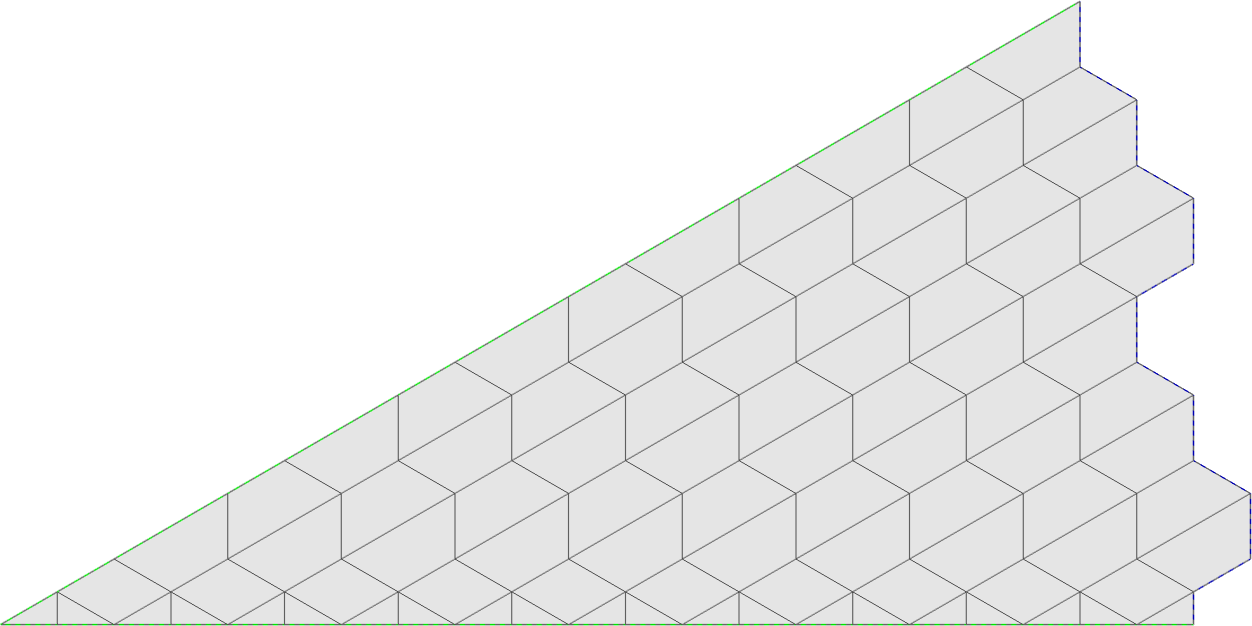
\includegraphics[scale=.2]{vver440/start_mesh}
  \caption{Initial mesh for the WWER-440 benchmark (reflective conditions on the diagonal and bottom line, vacuum
  conditions at the right boundary).}
  \label{fig:60}
\end{figure}

\begin{figure}[!ht]
\centering
\subfigure[$\phi^1$]{
  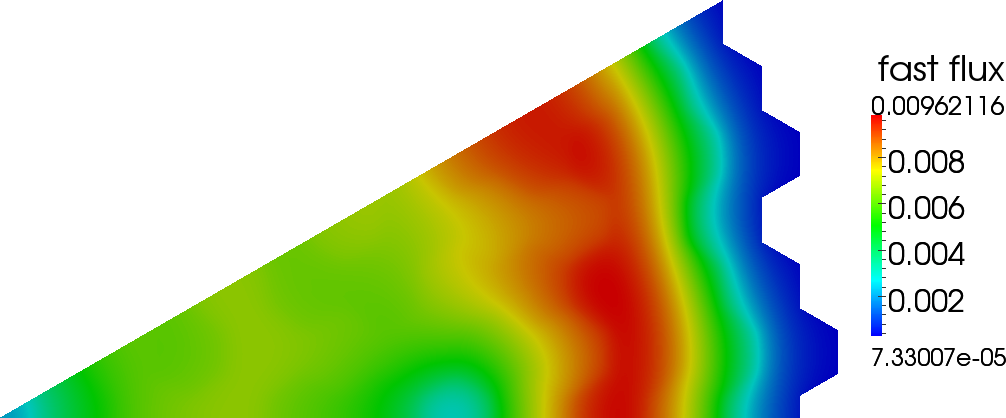
\includegraphics[scale=.275]{vver440/gg1.png}
}
\\[1em]
\subfigure[$\phi^2$]{
  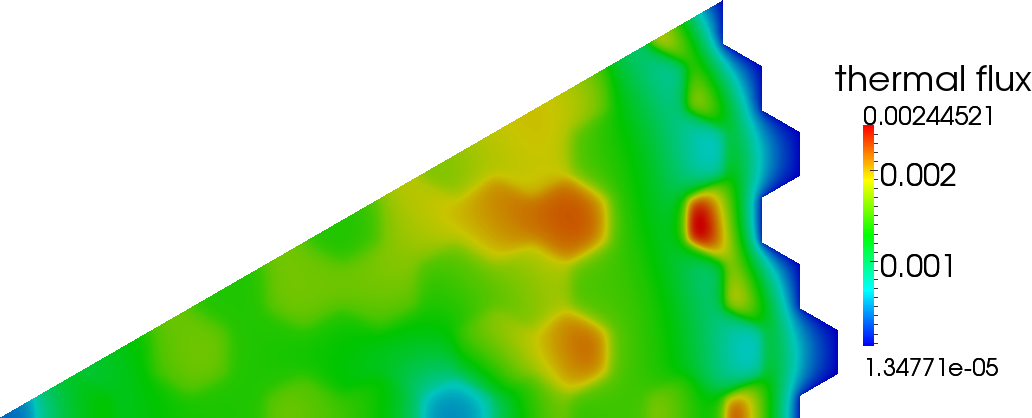
\includegraphics[scale=.275]{vver440/gg2.png}
}
  \caption[Solution of the WWER-440 benchmark]{Solution of the WWER-440 benchmark (group scalar fluxes).}
  \label{fig:61}
\end{figure}
\begin{figure}[!hb]
\centering
\subfigure[$g = 1$]{
  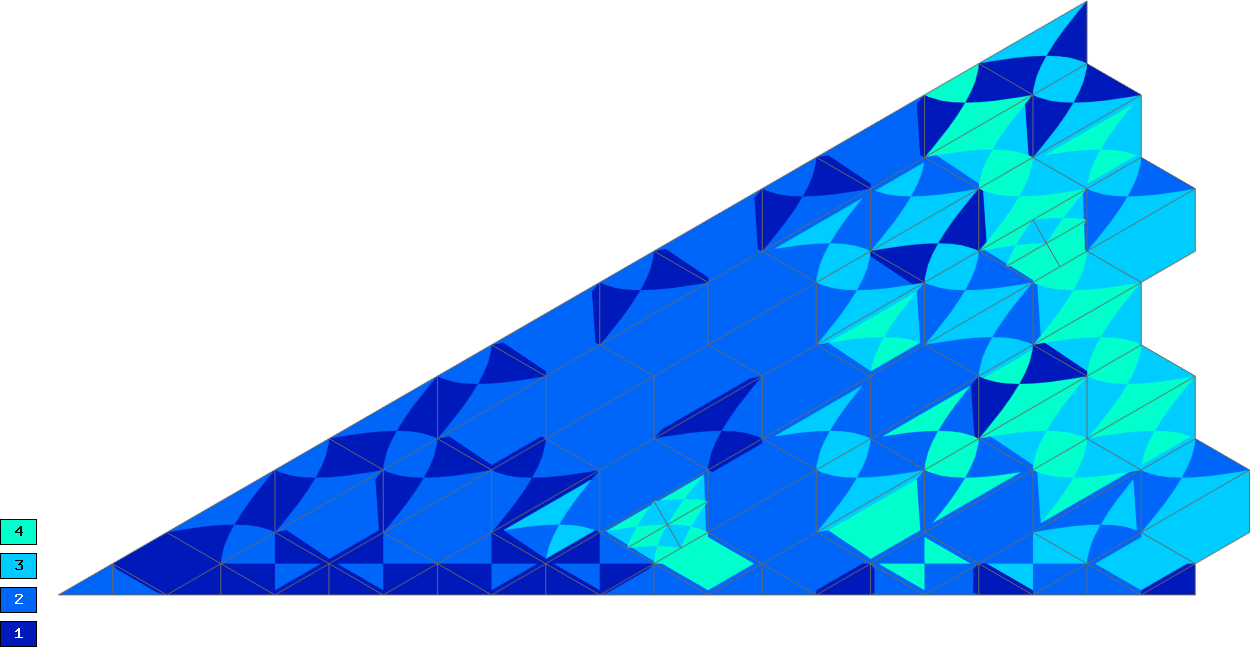
\includegraphics[scale=.2]{vver440/mesh_g1.png}
}
\\[.5em]
\subfigure[$g = 2$]{
  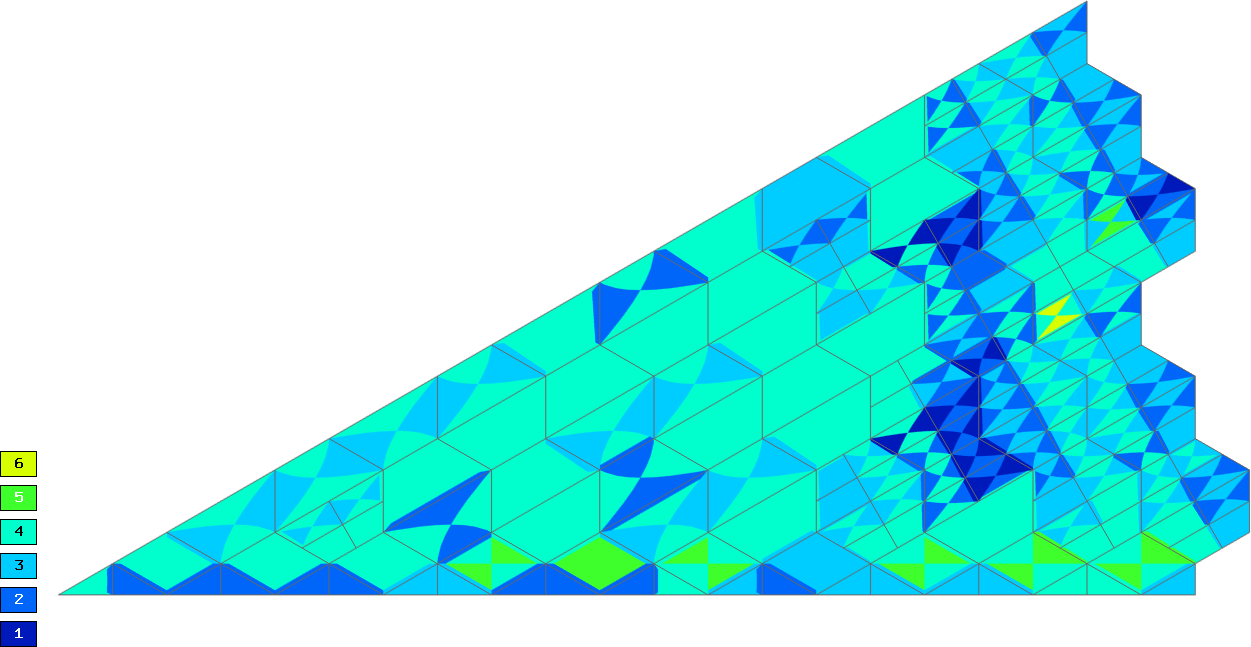
\includegraphics[scale=.2]{vver440/mesh_g2.png}
}
  \caption[Approximation spaces in the WWER-440 benchmark]{Approximation spaces for the WWER-440 benchmark.}
  \label{fig:62}
\end{figure}

\begin{figure}[!hb]
\centering
  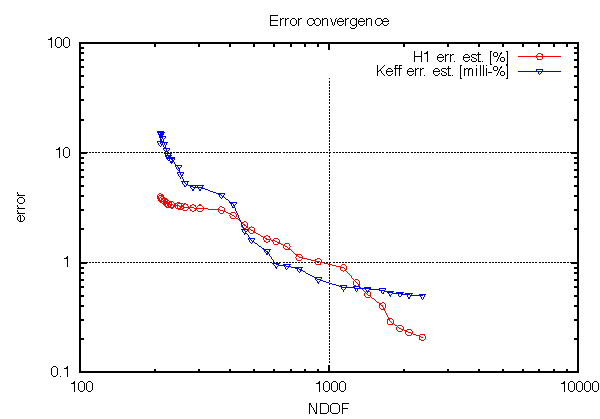
\includegraphics[scale=.85]{vver440/conv_dof}
  \caption[Adaptivity convergence curves for the WWER-440 benchmark]{Adaptivity convergence curves for the WWER-440
  benchmark. The reference value $\keff = 1.00970$ provided by \cite{Chao2}.}
  \label{fig:63}
\end{figure}

\clearpage
\subsubsection{Four-group VHTR criticality benchmark (diffusion)}
This benchmark of the criticality calculations in the azimuthally symmetric cylindrical geometry ($r-z$) has already
been implemented in Hermes2D as a stand-alone example when the author of this thesis joined the project. 
\begin{figure}[!htb]
\begin{center}
  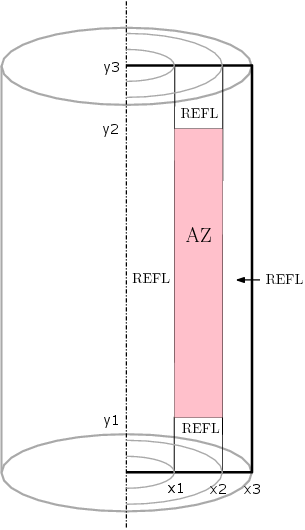
\includegraphics[scale=.4]{vhtr/VHTR}
  \caption[Geometry of the VHTR benchmark]{Geometry of the VHTR benchmark. Bold line encloses the rectangular region
  defining a computational domain for Hermes2D; vacuum boundary conditions are applied at these lines, while reflective
  condition is applied at the dash-dotted line. 
  $x1 = \SI{148}{cm}$,
  $x2 = \SI{242}{cm}$,
$x3 = \SI{340}{cm}$,
$y1 = \SI{158.5}{cm}$,
$y2 = \SI{951.5}{cm}$}
  \label{fig:70}
\end{center}
\end{figure}
It served as one example of
multimesh $hp$-adaptivity in \cite{Hermes-nuclear}. Identifying $r = x$, $z = y$, the problem is conveniently placed
into the Cartesian $x$-$y$ system (gradient components stay the same, while all
integrands need to be multiplied by $2\pi x$, i.e. the Jacobian determinant of the transformation between
Cartesian and cylindrical coordinates). We remark that this holds also for the integrals comprising the orthogonal
projection and error calculation forms used during adaptivity (which was not taken into account in the original
implementation, leading to less optimal convergence results).



The results of the new version implemented in the neutronics
framework and a more recent version of Hermes2D show the progress in the $hp$-adaptivity algorithms and
implementation -- while 27903 degrees of freedom were required to reach $(H^1)^4$ error estimate of 0.0164\% in
\cite{Hermes-nuclear}, only 21010 degrees of freedom on the final globally refined space were required in the new
version to reach comparable error estimate of 0.0172\% (the corresponding coarse space solution had 5010 degrees of
freedom as seen in \fref{fig:73}).

\begin{figure}[!ht]
\centering
\subfigure[$\phi^1$]{
  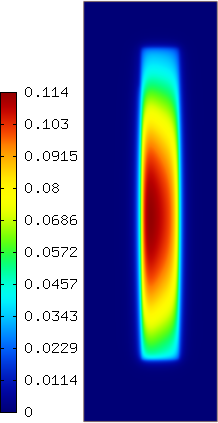
\includegraphics[scale=.36]{vhtr/gg1.png}
}
\hspace{.5em}
\subfigure[$\phi^2$]{
  \includegraphics[scale=.36]{vhtr/gg2.png}
}
\hspace{.5em}
\subfigure[$\phi^3$]{
  \includegraphics[scale=.36]{vhtr/gg3.png}
}
\hspace{.5em}
\subfigure[$\phi^4$]{
  \includegraphics[scale=.36]{vhtr/gg4.png}
}
  \caption[Solution of the VHTR benchmark]{Solution of the VHTR benchmark (group scalar fluxes).}
  \label{fig:71}
\end{figure}
\begin{figure}[!ht]
\centering
\subfigure[$g = 1$]{
  \includegraphics[scale=.36]{vhtr/mesh_g1.png}
}
\hspace{2em}
\subfigure[$g = 2$]{
  \includegraphics[scale=.36]{vhtr/mesh_g2.png}
}
\hspace{2em}
\subfigure[$g = 3$]{
  \includegraphics[scale=.36]{vhtr/mesh_g3.png}
}
\hspace{2em}
\subfigure[$g = 4$]{
  \includegraphics[scale=.36]{vhtr/mesh_g4.png}
}
  \caption[Approximation spaces in the VHTR benchmark]{Approximation spaces in the VHTR benchmark.}
  \label{fig:72} 
\end{figure}

\begin{figure}[!htb]
\begin{center}
  \includegraphics[scale=1]{vhtr/conv_dof}
  \caption[Adaptivity convergence curves for the VHTR benchmark]{Adaptivity convergence curves for the VHTR benchmark.
  The reference $\keff$ value 1.1409144 was obtained by a reference calculation on a 3x uniformly refined mesh with uniform distribution of polynomial degrees (=4), with power method and convergence
tolerance set to 5e-11. It slightly differs from the value 1.14077 reported in \cite{Hermes-nuclear}, where it is not
clear, however, how the value was obtained.}
  \label{fig:73}
\end{center}
\end{figure}


\subsection{$\SN$ examples}\label{sec:snex}

\subsubsection{Problem with exact solution}
To verify the implementation of the $\SN$ module, a simple solution
\begin{equation}\label{eq:1sol}
	\psi(\br,\bomega) = \psi(x,y,\Omega_x,\Omega_y) = \left
 \{ 
\begin{array}{cc}
 x y & \Omega _x>0\land \Omega _y>0 \\
 (1-x) y & \Omega _x<0\land \Omega _y>0 \\
 (1-x) (1-y) & \Omega _x<0\land \Omega _y<0 \\
 x (1-y) & \Omega _x>0\land \Omega _y<0 \\
\end{array}
 \right.
\end{equation}
has been manufactured for the following two-dimensional transport
problem with isotropic scattering constant throughout a unit-square domain enclosed by vacuum:
\begin{equation*}
    \bomega\cdot\nabla\psi(\br,\bomega) + \sigma_t\psi(\br,\bomega) -
    \frac{\sigma_s}{4\pi} \psi(\br,\bomega') =
    q(\br,\bomega),
\end{equation*}
yielding the following source term: 
$$
\begin{multlined}
q(\br,\bomega) =
\Omega _x \left(
\begin{array}{cc}
 y-1 & \Omega _x<0\land \Omega _y<0 \\
 1-y & \Omega _x>0\land \Omega _y<0 \\
 -y & \Omega _x<0\land \Omega _y>0 \\
 y & \Omega _x>0\land \Omega _y>0 \\
\end{array}
\right)+\Omega _y \left(
\begin{array}{cc}
 x-1 & \Omega _x<0\land \Omega _y<0 \\
 1-x & \Omega _x<0\land \Omega _y>0 \\
 -x & \Omega _x>0\land \Omega _y<0 \\
 x & \Omega _x>0\land \Omega _y>0 \\
\end{array}
\right)\\[.5em]
- \frac{\sigma _s}{4\pi}+\sigma _t \left(
\begin{array}{cc}
 x y & \Omega _x>0\land \Omega _y>0 \\
 (1-x) y & \Omega _x<0\land \Omega _y>0 \\
 (1-x) (1-y) & \Omega _x<0\land \Omega _y<0 \\
 x (1-y) & \Omega _x>0\land \Omega _y<0 \\
\end{array}
\right).
\end{multlined}
$$
It is easy to see that
$$
	\phi(\br) = \intA{\psi(\br,\bomega)} = \pi.
$$
An exact solution $\psi(\br,\bomega)$ with $\bomega = \frac{\sqrt{2}}{2} [1,1]^T$ corresponding to the azimuthal
angle $\azimuthal = 45^\circ$ has been computed by Mathematica and is shown in \fref{fig:10}.

\begin{figure}[!ht]
\centering
  \includegraphics[scale=.275]{exact/exact}
  \caption[Manufactured solution problem]{Manufactured solution problem -- exact $\psi_1$.}
  \label{fig:10}
\end{figure}

Solution by Hermes2D for
an arbitrary set of cross-sections $\sigma_t = \SI{1}{cm^{-1}}$, $\sigma_s = \SI{0.5}{cm^{-1}}$ is presented in figures
\ref{fig:11} (scalar flux) and \ref{fig:12} to (angular fluxes in first four directions of the $\SN[4]$ set; same set of solutions 
have been obtained in the remaining directions, as expected from \eqref{eq:1sol}). 
\begin{figure}[!ht]
\centering
  \includegraphics[scale=.2]{exact/phi-conv}
  \caption[Manufactured solution problem -- converged scalar flux]{Manufactured solution problem -- converged scalar
  flux.}
  \label{fig:11}
\end{figure}

\begin{figure}[!ht]
\centering
\subfigure[$\psi_1$]{
  \includegraphics[scale=.185]{exact/psi1.png}
}
\hspace{1em}
\subfigure[$\psi_2$]{
  \includegraphics[scale=.185]{exact/psi2.png}
}
%\label{fig:12} 
\end{figure}
\begin{figure}[h!]
\ContinuedFloat
\centering
%\hspace{.1em}
\subfigure[$\psi_3$]{
  \includegraphics[scale=.185]{exact/psi3.png}
}
\hspace{1em}
\subfigure[$\psi_4$]{
  \includegraphics[scale=.185]{exact/psi4.png}
}
  \caption[Manufactured solution problem -- converged angular fluxes]{Manufactured solution problem -- converged angular
  fluxes in first direction within each quadrant.}
  \label{fig:12} 
\end{figure}

Note that although the solution does 
not depend on the choice of $\sigma_t$ and $\sigma_s$, $c = \sigma_s / \sigma_t$ will influence the convergence rate of 
the source iteration process implemented in Hermes2D, as noted in \sref{sec:SI}.
Figure \ref{fig:11} shows the solution of source iteration converged with tolerance $10^{-10}$ (19 iterations),
while the solution converged with tolerance $10^{-5}$ (9 iterations) is shown in \fref{fig:16}. As indicated by
Theorem \ref{thm:3}, the convergence rate depends on the product $c\sigma_t = \sigma_s$; 17 iterations were needed to
converge the solution for $\sigma_t = \SI{100}{cm^{-1}}$, $\sigma_s = \SI{50}{cm^{-1}}$ with the tolerance set to the
same value $10^{-5}$ (Figure \ref{fig:17}).

\begin{figure}[!ht]
\centering
  \includegraphics[scale=.24]{exact/phi}
  \caption[Manufactured solution problem -- scalar flux]{Manufactured solution problem -- scalar
  flux from angular fluxes converged to within tolerance $10^{-5}$.}
  \label{fig:16}
\end{figure}

\begin{figure}[!ht]
\centering
  \includegraphics[scale=.2]{exact/phi2}
  \caption[Manufactured solution problem -- scalar flux]{Manufactured solution problem -- scalar
  flux from angular fluxes converged to within tolerance $10^{-5}$ (different cross-section set).}
  \label{fig:17}
\end{figure} 

\subsubsection{Watanabe-Maynard Problem 1}\label{sec:wm1}
This benchmark has been presented in \cite{watanabe} to demonstrate ray-effect mitigation (see \sref{sec:SN_advection})
of the special methods developed in the paper. A uniform isotropic source is placed at the center of a
vacuum-surrounded domain and separated from the scattering part of the domain by a layer of vacuum as illustrated in
\fref{fig:20}. 

\begin{figure}[!htb]
\centering
  \includegraphics[scale=.4]{wm1/WM}
  \caption[Watanabe-Maynard problem]{Geometry and reference solutions of the Watanabe-Maynard problem (from
  \cite{watanabe}). Source strength is \SI{6.4}{cm^{-3}.sec}.}
  \label{fig:20}
\end{figure}

\begin{figure}[!ht]
\centering
  \includegraphics[scale=.42]{wm1/DRAGONl}\\
  \includegraphics[scale=.25]{wm1/DRAGON}
  \caption{Solution of the Watanabe-Maynard problem by DRAGON. Values span the range $[3.57\times 10^{-1},
  15.537]$.}
  \label{fig:24}
\end{figure}

While the ray-effects are clearly present in our $\SN[8]$ solution (figures \ref{fig:22}, \ref{fig:23}),
which has not been treated to diminish these oscillations in any special way, these appear to be less pronounced than
when using the standard $\SN[8]$ ordinates set (line ``S8'' in \fref{fig:20}). 

\begin{figure}[!ht]
\centering
\subfigure[scalar flux]{
  \includegraphics[scale=.2]{wm1/phi.png}
}
\subfigure[scalar flux at $x = \SI{5.625}{cm}$]{
  \includegraphics[scale=.2]{wm1/R3P1-S8}
}
  \caption[Solution of the Watanabe-Maynard problem]{Solution of the Watanabe-Maynard problem, using the mesh from
  \fref{fig:24} with one level of uniform refinement and $DG(0)$ elements.}
  \label{fig:22}
\end{figure}

Note also that ray effects become more
visible when refining the mesh (\fref{fig:23}), confirming the importance of keeping the mesh refinement in harmony with
the increase of the number of directions. For comparison, \fref{fig:24} shows the solution provided by the code DRAGON
using the method of characteristics using the setup from \cite[Sec. 6.4.3]{dragon}. % SAME MESH AS FOR FIG22.

\begin{figure}[!ht]
\centering
\subfigure[scalar flux]{
  \includegraphics[scale=.2]{wm1/phi2.png}
}
\subfigure[scalar flux at $x = \SI{5.625}{cm}$]{
  \includegraphics[scale=.2]{wm1/R4P1-S8}
}
  \caption[Solution of the Watanabe-Maynard problem -- refined mesh]{Solution of the Watanabe-Maynard problem, using
   the mesh from \fref{fig:24} with two levels of uniform refinements and $DG(0)$ elements.}
  \label{fig:23}
\end{figure}


\section{Coupled code system for quasi-static whole-core calculations}\label{sec:coupled}

A fully three-dimensional multigroup neutron diffusion solver was needed for the purposes of
the project ``Project TA01020352 -- Increasing utilization of nuclear fuel through optimization of an inner fuel cycle
and calculation of neutron-physics characteristics of nuclear reactor cores'', which the author of this thesis
participated in during his doctoral studies. As the 3D version of Hermes has not been released yet, another
finite-element library has been chosen and the experience obtained from developing the neutronics solvers within
Hermes2D was utilized to develop a similar framework using this library as a backend. Namely, the FE matrix assembly is
handled by the well-established open-source system FEniCS \cite{dolfin1, dolfin2} and its linear algebra backend PETSc \cite{petsc1}. PETSc library and its fork focusing on solving large sparse
eigenvalue problems, SLEPc \cite{slepc1}, is also primarily used for solving the assembled algebraic problems (mainly
the generalized eigenvalue problems of form \eqref{eq:discrete_eigenproblem} that are of most importance in this
project; cf. also the introduction to \sref{sec:criticality}). This has the advantage that parallel assembly and
solution using MPI is almost automatic (provided an appropriate solver/preconditioner is being used). %FEniCS also makes it easy to pass arguments directly to the linear-algebra
%backend, thus facilitating for the user the selection of algebraic solver and its properties. 

\begin{figure}[p]
\centering
  \includegraphics[scale=.55]{schema}
  \caption[Coupled code run scheme]{Coupled code run scheme.}
  \label{fig:scheme}
\end{figure}

The code operates along the scheme shown in \fref{fig:scheme} and is written in Python 2.7
with critical parts (typically where loops over mesh cells are needed) in C++ as SWIG extension modules. The
ability to mix Python with C++ extensions as well as availability of Python modules that can achieve C++-like
performance if used in an appropriate way (Numpy for operations with large data arrays, mpi4py for MPI-related tasks)
make the code sufficiently fast and flexible at the same time.
Thorough description of the code and its 
results on standard industry benchmarks formed the content of three research reports 
that were accepted by the project issuing agency (one final report is currently in preparation). To keep the scope of
this thesis reasonable, just a sample of these results for one such benchmark -- the steady-state part of the OECD/NEA
MOX-UO2 benchmark \cite{mox-bench} -- is presented below to provide an example of the capabilities of the code. 

\begin{table}[b]
\begin{tabular}{|c|c|c|c|c|c|c|c|}
\hline  & \%PWE & $c_b$ & $T_D$ & $\rho_m$ & $T_m$ & $\rho_m^o$ & $T_m^o$ \\ 
\hline \textsl{CORETRAN} & 0.31 & 1647 & 908.4 & 706.1 & 581.0 & 658.5 & 598.6 \\ 
\hline \textsl{CORETRAN 4/FA} & 0.26 & 1645 & 908.4 & 706.1 & 581.0 & 658.5 & 598.6 \\ 
\hline \textsl{EPISODE} & 0.40 & 1661 & 846.5 & 701.8 & 582.6 & 697.4 & 585.5 \\ 
\hline \textsl{NUREC} & 0.31 & 1683 & 827.8 & 706.1 & 581.1 & 661.5 & 598.7 \\ 
\hline \textsl{PARCS2G} & ref & 1679 & 836.0 & 706.1 & 581.3 & 662.1 & 598.8 \\ 
\hline \textsl{SKETCH-INS} & 1.04 & 1675 & 836.6 & 705.5 & 580.9 & 659.6 & 598.9 \\ 
\hline\hline Results & 1.35 & 1699 & 839.0 & 702.1 & 582.3 & 660.1 & 599.1 \\ 
\hline 
\end{tabular}
\caption[OECD/NEA MOX-UO2 benchmark -- comparison with various nodal methods]{
OECD/NEA MOX-UO2 benchmark (hot full power case) -- comparison of results with various nodal methods from
\cite{mox-bench}.\\
$
 	PWE = \frac{\sum_{a\in\text{assemblies}}\lvert P_{a} - P^{\text{ref}}_{a} \rvert P^{\text{ref}}_{a}}
 			   {\sum_{a\in\text{assemblies}} P^{\text{ref}}_{a}},\quad P_a\ldots\mbox{ assembly integrated power } 
$
\index{Pa@$P_a$|see {power density}}
}
\end{table} 

The problem was solved using the Jacobi-Davidson generalized eigensolver (\cite{slepcjd}) with a PETSc implementation of
BiCGStab($\ell$) \cite{Sleijpen1} as an inner solver (using the default $\ell = 2$). It has been demonstrated already in \cite{Sleijpen1} (and analyzed in many later papers, see
e.g. \cite{Notay} and references therein) that the Jacobi-Davidson method is remarkably robust with respect to accuracy
of the solution of the inner solution phase. Therefore, by setting a fixed number of inner iterations to 20 and
employing a smoothed aggregation algebraic multigrid preconditioner with 1 pre- and 1 post-smoothing Richardson
iterations, eigenvalue convergence within at most 10 outer iterations was achieved in every feedback step. 34 feedback
iterations were required in the hot full power calculation to converge all fields of interest to within $10^{-4}$
relative difference from previous iteration, leading to a total calculation time of 1053 seconds. 

\begin{figure}[!ht]
\centering
  \includegraphics[width=.7\textwidth]{mox/mesh}
  \caption[Mesh for the OECD/NEA MOX-UO2 benchmark]{Mesh for the OECD/NEA MOX-UO2 benchmark (generated by GMSH
  \cite{GMSH}).  Colored by regions that can be assigned different neutronic/TH properties (i.e., fuel pins in the
  core interior; note that assembly-homogenized cross-sections are given in the benchmark, but T/H feedbacks are
  actually calculated pin-by-pin.}
\end{figure}

\begin{figure}[!ht]
\centering
  \includegraphics[width=.335\textwidth]{mox/rank-ass}\hspace{2em}
  \includegraphics[width=.5\textwidth]{mox/rank-th}
  \caption[Parallel mesh distribution in the OECD/NEA MOX-UO2 benchmark]{Mesh distribution on 12 CPUs -- automatic
  distribution by the SCOTCH library (used by FEniCS for assembling the FE matrices) on left, manual redistribution
  for efficient parallel T/H calculations on right (i.e., complete axial channels from core inlet to outlet are
  available at each processor).}
  \label{fig:mox2}
\end{figure}



\begin{figure}[!hb]
\centering
\subfigure[hot zero power case]{
  \includegraphics[scale=.3]{mox/power_hzp}
}
\label{fig:mox4}
\end{figure}
\begin{figure}[!ht]
\ContinuedFloat
\centering
\subfigure[hot full power case]{
  \includegraphics[scale=.15]{mox/power_hfp}
}
  \caption{Core-wide power distribution.}
  \label{fig:mox5}
\end{figure}


\begin{figure}[!htb]
\centering
  \includegraphics[scale=.18]{mox/Tf}
  \includegraphics[scale=.18]{mox/Tm}
  \caption{T/H fields distribution.}
  \label{fig:mox6}
\end{figure}

\begin{figure}[p]
\centering
\subfigure[hot zero power case]{
  \includegraphics[scale=.4]{mox/axial}
}
\hspace{1em}
\subfigure[hot full power case]{
  \includegraphics[scale=.4]{mox/axial-hfp}
}
  \caption{Axial power distribution.}
  \label{fig:mox3}
\end{figure}
